\documentclass[a4paper]{article}

\def\npart {III}
\def\nterm {Michaelmas}
\def\nyear {2017}
\def\nlecturer {B. Bollobas}
\def\ncourse {Combinatorics}

% Imports
\ifx \nextra \undefined
  \usepackage[pdftex,
    hidelinks,
    pdfauthor={Dexter Chua},
    pdfsubject={Cambridge Maths Notes: Part \npart\ - \ncourse},
    pdftitle={Part \npart\ - \ncourse},
  pdfkeywords={Cambridge Mathematics Maths Math \npart\ \nterm\ \nyear\ \ncourse}]{hyperref}
  \title{Part \npart\ - \ncourse}
\else
  \usepackage[pdftex,
    hidelinks,
    pdfauthor={Dexter Chua},
    pdfsubject={Cambridge Maths Notes: Part \npart\ - \ncourse\ (\nextra)},
    pdftitle={Part \npart\ - \ncourse\ (\nextra)},
  pdfkeywords={Cambridge Mathematics Maths Math \npart\ \nterm\ \nyear\ \ncourse\ \nextra}]{hyperref}

  \title{Part \npart\ - \ncourse \\ {\Large \nextra}}
\fi

\author{Lectured by \nlecturer \\\small Notes taken by Dexter Chua}
\date{\nterm\ \nyear}

\usepackage{alltt}
\usepackage{amsfonts}
\usepackage{amsmath}
\usepackage{amssymb}
\usepackage{amsthm}
\usepackage{booktabs}
\usepackage{caption}
\usepackage{enumitem}
\usepackage{fancyhdr}
\usepackage{graphicx}
\usepackage{mathtools}
\usepackage{microtype}
\usepackage{multirow}
\usepackage{pdflscape}
\usepackage{pgfplots}
\usepackage{siunitx}
\usepackage{tabularx}
\usepackage{tikz}
\usepackage{tkz-euclide}
\usepackage[normalem]{ulem}
\usepackage[all]{xy}

\pgfplotsset{compat=1.12}

\pagestyle{fancyplain}
\lhead{\emph{\nouppercase{\leftmark}}}
\ifx \nextra \undefined
  \rhead{
    \ifnum\thepage=1
    \else
      \npart\ \ncourse
    \fi}
\else
  \rhead{
    \ifnum\thepage=1
    \else
      \npart\ \ncourse\ (\nextra)
    \fi}
\fi
\usetikzlibrary{arrows}
\usetikzlibrary{decorations.markings}
\usetikzlibrary{decorations.pathmorphing}
\usetikzlibrary{positioning}
\usetikzlibrary{fadings}
\usetikzlibrary{intersections}
\usetikzlibrary{cd}

\newcommand*{\Cdot}{\raisebox{-0.25ex}{\scalebox{1.5}{$\cdot$}}}
\newcommand {\pd}[2][ ]{
  \ifx #1 { }
    \frac{\partial}{\partial #2}
  \else
    \frac{\partial^{#1}}{\partial #2^{#1}}
  \fi
}

% Theorems
\theoremstyle{definition}
\newtheorem*{aim}{Aim}
\newtheorem*{axiom}{Axiom}
\newtheorem*{claim}{Claim}
\newtheorem*{cor}{Corollary}
\newtheorem*{defi}{Definition}
\newtheorem*{eg}{Example}
\newtheorem*{fact}{Fact}
\newtheorem*{law}{Law}
\newtheorem*{lemma}{Lemma}
\newtheorem*{notation}{Notation}
\newtheorem*{prop}{Proposition}
\newtheorem*{thm}{Theorem}

\renewcommand{\labelitemi}{--}
\renewcommand{\labelitemii}{$\circ$}
\renewcommand{\labelenumi}{(\roman{*})}

\let\stdsection\section
\renewcommand\section{\newpage\stdsection}

% Strike through
\def\st{\bgroup \ULdepth=-.55ex \ULset}

% Maths symbols
\newcommand{\bra}{\langle}
\newcommand{\ket}{\rangle}

\newcommand{\N}{\mathbb{N}}
\newcommand{\Z}{\mathbb{Z}}
\newcommand{\Q}{\mathbb{Q}}
\renewcommand{\H}{\mathbb{H}}
\newcommand{\R}{\mathbb{R}}
\newcommand{\C}{\mathbb{C}}
\newcommand{\Prob}{\mathbb{P}}
\renewcommand{\P}{\mathbb{P}}
\newcommand{\E}{\mathbb{E}}
\newcommand{\F}{\mathbb{F}}
\newcommand{\cU}{\mathcal{U}}
\newcommand{\RP}{\mathbb{RP}}
\newcommand{\CP}{\mathbb{CP}}

\newcommand{\ph}{\,\cdot\,}

\DeclareMathOperator{\sech}{sech}
\DeclareMathOperator{\cosech}{cosech}
\DeclareMathOperator{\cosec}{cosec}

\DeclareMathOperator{\covol}{covol}
\DeclareMathOperator{\vol}{vol}

\let\Im\relax
\let\Re\relax
\DeclareMathOperator{\Im}{Im}
\DeclareMathOperator{\Re}{Re}
\DeclareMathOperator{\im}{im}
\DeclareMathOperator{\image}{image}
\DeclareMathOperator{\Ann}{Ann}

\DeclareMathOperator*{\res}{res}
\DeclareMathOperator{\Res}{Res}
\DeclareMathOperator{\Ind}{Ind}

\DeclareMathOperator{\tr}{tr}
\DeclareMathOperator{\diag}{diag}
\DeclareMathOperator{\rank}{rank}
\DeclareMathOperator{\card}{card}
\DeclareMathOperator{\spn}{span}
\DeclareMathOperator{\adj}{adj}

\DeclareMathOperator{\erf}{erf}
\DeclareMathOperator{\erfc}{erfc}

\DeclareMathOperator{\ord}{ord}
\DeclareMathOperator{\Sym}{Sym}

\DeclareMathOperator{\sgn}{sgn}
\DeclareMathOperator{\orb}{orb}
\DeclareMathOperator{\stab}{stab}
\DeclareMathOperator{\ccl}{ccl}

\DeclareMathOperator{\lcm}{lcm}
\DeclareMathOperator{\hcf}{hcf}

\DeclareMathOperator{\Int}{Int}
\DeclareMathOperator{\id}{id}

\DeclareMathOperator{\betaD}{beta}
\DeclareMathOperator{\gammaD}{gamma}
\DeclareMathOperator{\Poisson}{Poisson}
\DeclareMathOperator{\binomial}{binomial}
\DeclareMathOperator{\multinomial}{multinomial}
\DeclareMathOperator{\Bernoulli}{Bernoulli}
\DeclareMathOperator{\like}{like}

\DeclareMathOperator{\var}{var}
\DeclareMathOperator{\cov}{cov}
\DeclareMathOperator{\bias}{bias}
\DeclareMathOperator{\mse}{mse}
\DeclareMathOperator{\corr}{corr}

\DeclareMathOperator{\otp}{otp}
\DeclareMathOperator{\dom}{dom}

\DeclareMathOperator{\Root}{Root}
\DeclareMathOperator{\supp}{supp}
\DeclareMathOperator{\rel}{rel}
\DeclareMathOperator{\Hom}{Hom}
\DeclareMathOperator{\Aut}{Aut}
\DeclareMathOperator{\Gal}{Gal}
\DeclareMathOperator{\Mat}{Mat}
\DeclareMathOperator{\End}{End}
\DeclareMathOperator{\Char}{char}
\DeclareMathOperator{\ev}{ev}
\DeclareMathOperator{\St}{St}
\DeclareMathOperator{\Lk}{Lk}
\DeclareMathOperator{\disc}{disc}
\DeclareMathOperator{\Isom}{Isom}
\DeclareMathOperator{\length}{length}
\DeclareMathOperator{\energy}{energy}
\DeclareMathOperator{\area}{area}
\DeclareMathOperator{\Syl}{Syl}
\DeclareMathOperator{\cl}{cl}
\DeclareMathOperator{\fix}{fix}

\newcommand{\GL}{\mathrm{GL}}
\newcommand{\SL}{\mathrm{SL}}
\newcommand{\PGL}{\mathrm{PGL}}
\newcommand{\PSL}{\mathrm{PSL}}
\newcommand{\PSU}{\mathrm{PSU}}
\newcommand{\Or}{\mathrm{O}}
\newcommand{\SO}{\mathrm{SO}}
\newcommand{\U}{\mathrm{U}}
\newcommand{\SU}{\mathrm{SU}}

\renewcommand{\d}{\mathrm{d}}
\newcommand{\D}{\mathrm{D}}

\tikzset{->/.style = {decoration={markings,
                                  mark=at position 1 with {\arrow[scale=2]{latex'}}},
                      postaction={decorate}}}
\tikzset{<-/.style = {decoration={markings,
                                  mark=at position 0 with {\arrowreversed[scale=2]{latex'}}},
                      postaction={decorate}}}
\tikzset{<->/.style = {decoration={markings,
                                   mark=at position 0 with {\arrowreversed[scale=2]{latex'}},
                                   mark=at position 1 with {\arrow[scale=2]{latex'}}},
                       postaction={decorate}}}
\tikzset{->-/.style = {decoration={markings,
                                   mark=at position #1 with {\arrow[scale=2]{latex'}}},
                       postaction={decorate}}}
\tikzset{-<-/.style = {decoration={markings,
                                   mark=at position #1 with {\arrowreversed[scale=2]{latex'}}},
                       postaction={decorate}}}

\tikzset{circ/.style = {fill, circle, inner sep = 0, minimum size = 3}}
\tikzset{mstate/.style={circle, draw, blue, text=black, minimum width=0.7cm}}

\definecolor{mblue}{rgb}{0.2, 0.3, 0.8}
\definecolor{morange}{rgb}{1, 0.5, 0}
\definecolor{mgreen}{rgb}{0.1, 0.4, 0.2}
\definecolor{mred}{rgb}{0.5, 0, 0}

\def\drawcirculararc(#1,#2)(#3,#4)(#5,#6){%
    \pgfmathsetmacro\cA{(#1*#1+#2*#2-#3*#3-#4*#4)/2}%
    \pgfmathsetmacro\cB{(#1*#1+#2*#2-#5*#5-#6*#6)/2}%
    \pgfmathsetmacro\cy{(\cB*(#1-#3)-\cA*(#1-#5))/%
                        ((#2-#6)*(#1-#3)-(#2-#4)*(#1-#5))}%
    \pgfmathsetmacro\cx{(\cA-\cy*(#2-#4))/(#1-#3)}%
    \pgfmathsetmacro\cr{sqrt((#1-\cx)*(#1-\cx)+(#2-\cy)*(#2-\cy))}%
    \pgfmathsetmacro\cA{atan2(#2-\cy,#1-\cx)}%
    \pgfmathsetmacro\cB{atan2(#6-\cy,#5-\cx)}%
    \pgfmathparse{\cB<\cA}%
    \ifnum\pgfmathresult=1
        \pgfmathsetmacro\cB{\cB+360}%
    \fi
    \draw (#1,#2) arc (\cA:\cB:\cr);%
}
\newcommand\getCoord[3]{\newdimen{#1}\newdimen{#2}\pgfextractx{#1}{\pgfpointanchor{#3}{center}}\pgfextracty{#2}{\pgfpointanchor{#3}{center}}}

\def\Xint#1{\mathchoice
   {\XXint\displaystyle\textstyle{#1}}%
   {\XXint\textstyle\scriptstyle{#1}}%
   {\XXint\scriptstyle\scriptscriptstyle{#1}}%
   {\XXint\scriptscriptstyle\scriptscriptstyle{#1}}%
   \!\int}
\def\XXint#1#2#3{{\setbox0=\hbox{$#1{#2#3}{\int}$}
     \vcenter{\hbox{$#2#3$}}\kern-.5\wd0}}
\def\ddashint{\Xint=}
\def\dashint{\Xint-}


\begin{document}
\maketitle
{\small
\setlength{\parindent}{0em}
\setlength{\parskip}{1em}

What can one say about a collection of subsets of a finite set satisfying certain conditions in terms of containment, intersection and union? In the past fifty years or so, a good many fundamental results have been proved about such questions: in the course we shall present a selection of these results and their applications, with emphasis on the use of algebraic and probabilistic arguments.

The topics to be covered are likely to include the following:
\begin{itemize}
  \item The de Bruijn--Erd\"os theorem and its extensions.
  \item The Graham--Pollak theorem and its extensions.
  \item The theorems of Sperner, EKR, LYMB, Katona, Frankl and F\"uredi. % check Furedi
  \item Isoperimetric inequalities: Kruskal--Katona, Harper, Bernstein, BTBT, and their applications.
  \item Correlation inequalities, including those of Harris, van den Berg and Kesten, and the Four Functions Inequality.
  \item Alon's Combinatorial Nullstellensatz and its applications.
  \item LLLL and its applications.
\end{itemize}

\subsubsection*{Pre-requisites}
The main requirement is mathematical maturity, but familiarity with the basic graph theory course in Part II would be helpful.
}
\tableofcontents

\section{Hall's theorem}
We shall begin with a discussion of Hall's theorem. Ideally, you've already met it in IID Graph Theory, but we shall nevertheless go through it again.

\begin{defi}[Bipartite graph]\index{bipartite graph}
  We say $G = (X, Y; E)$ is a \emph{bipartite graph} with bipartition $X$ and $Y$ if $(X \sqcup Y, E)$ is a graph such that every edge is between a vertex in $X$ and a vertex in $Y$.

  We say such a bipartite graph is \term{$(k, \ell)$-regular} if every vertex in $X$ has degree $k$ and every vertex in $Y$ has degree $\ell$. A bipartite graph that is $(k, \ell)$-regular for some $k, \ell \geq 1$ is said to be \emph{biregular}\index{biregular graph}.
\end{defi}

\begin{defi}[Complete matching]\index{complete matching}
  Let $G = (X, Y; E)$ be a bipartite graph with bipartition $X$ and $Y$. A \emph{complete matching} from $X$ to $Y$ is an injection $f: X \to Y$ such that $x\, f(x)$ is an edge for every $x \in X$.
\end{defi}

Hall's theorem gives us a necessary and sufficient condition for the existence of a complete matching. Let's try to first come up with a necessary condition. If there is a complete matching, then for any subset $S \subseteq X$, we certainly have $|\Gamma(S)| \geq |S|$, where \term{$\Gamma(S)$} is the set of neighbours of $S$. Hall's theorem says this is also sufficient.

\begin{thm}[Hall, 1935]\index{Hall's theorem}
  A bipartite graph $G = (X, Y; E)$ has a complete matching from $X$ to $Y$ if and only if $|\Gamma(S)| \geq |S|$ for all $S \subseteq X$.
\end{thm}
This condition is known as \term{Hall's condition}.

\begin{proof}
  We may assume $G$ is edge-minimal satisfying Hall's condition. We show that $G$ is a complete matching from $X$ to $Y$. For $G$ to be a complete matching, we need the following two properties:
  \begin{enumerate}
    \item Every vertex in $X$ has degree $1$
    \item Every vertex in $Y$ has degree $0$ or $1$.
  \end{enumerate}

  We first examine the second condition. Suppose $y \in Y$ is such that there exists edges $x_1 y, x_2 y \in E$. Then the minimality of $G$ implies there are sets, $X_1, X_2 \subseteq X$ such that $x_i \in X_i$ such that $|\Gamma(X_i)| = |X_i|$ and $x_i$ is the only neighbour of $y$ in $X_i$.

  Now consider the set $X_1 \cap X_2$. We know $\Gamma(X_1 \cap X_2) \subseteq \Gamma(X_1) \cap \Gamma(X_2)$. Moreover, this is strict, as $y$ is in the RHS but not the LHS. So we have
  \[
    \Gamma(X_1 \cap X_2) \leq |\Gamma(X_i) \cap \Gamma(X_2)| - 1.
  \]
  But also
  \begin{align*}
    |X_1 \cap X_2| &\leq |\Gamma(X_1 \cap X_2)|\\
    &\leq |\Gamma(X_1) \cap \Gamma(X_2)| - 1 \\
    &= |\Gamma(X_1)| + |\Gamma(X_2)| - |\Gamma(X_1) \cup \Gamma(X_2)| - 1\\
    &= |X_1| + |X_2| - |\Gamma(X_1\cup X_2)| - 1\\
    &\leq |X_1| + |X_2| - |X_1 \cup X_2| - 1\\
    &= |X_1 \cap X_2| - 1,
  \end{align*}
  which contradicts Hall's condition.

  One then sees that the first condition is also satisfied --- if $x \in X$ is a vertex, then the degree of $x$ certainly cannot be $0$, or else $|\Gamma(\{x\})| < |\{x\}|$, and we see that $d(x)$ cannot be $>1$ or else we can just remove an edge from $x$ without violating Hall's condition.
\end{proof}

We shall now describe some consequences of Hall's theorem. They will be rather straightforward applications, but we shall later see they have some interesting consequences.

Let $\mathcal{A} = \{A_1, \ldots, A_m\}$ be a set system. All sets are finite. A set of \term{distinct representatives} of $\mathcal{A}$ is a set $\{a_1, \ldots a_m\}$ of distinct elements $a_i \in A_i$.

Under what condition do we have a set of distinct representatives? If we have one, then for any $I \subseteq [m] = \{1, 2, \ldots, m\}$, we have
\[
  \left|\bigcup_{i \in I} A_i \right| \geq |I|.
\]
We might hope this is sufficient.
\begin{thm}
  $\mathcal{A}$ has a set of distinct representatives iff for all $\mathcal{B} \subseteq \mathcal{A}$, we have
  \[
    \left|\bigcup_{B \in \mathcal{B}} B\right| \geq |\mathcal{B}|.
  \]
\end{thm}

This is an immediate consequence of Hall's theorem.

\begin{proof}
  Define a bipartite graph as follows --- we let $X = \mathcal{A}$, and $Y = \bigcup_{i \in [m]} A_i$. Then draw an edge from $x$ to $A_i$ if $x \in A_i$. Then there is a complete matching of this graph iff $\mathcal{A}$ has a set of distinct representations, and the condition in the theorem is exactly Hall's condition. So we are done by Hall's theorem.
\end{proof}

\begin{thm}
  Let $G = (X, Y; E)$ be a bipartite graph such that $d(x) \geq d(y)$ for all $x \in X$ and $y \in Y$. Then there is a complete matching from $X$ to $Y$.
\end{thm}

\begin{proof}
  Let $d$ be such that $d(x) \geq d \geq d(y)$ for all $x \in X$ and $y \in Y$. For $S \subseteq X$ and $T \subseteq Y$, we let $e(S, T)$ be the number of edges between $S$ and $T$. Let $S \subseteq X$, and $T = \Gamma(S)$. Then we have
  \[
    e(S, T) = \sum_{x \in S} d(x) \geq d |S|,
  \]
  but on the other hand, we have
  \[
    e(S, T) \leq \sum_{y \in T} d(y) \leq d |T|.
  \]
  So we find that $|T| \geq |S|$. So Hall's condition is satisfied.
\end{proof}

\begin{cor}
  If $G = (X, Y; E)$ is a $(k, \ell)$-regular bipartite graph with $1 \leq \ell \leq k$, then there is a complete matching from $X$ to $Y$.
\end{cor}

\begin{thm}
  Let $G = (X, Y; E)$ be biregular and $A \subseteq X$. Then
  \[
    \frac{|\Gamma(A)|}{|Y|}\geq \frac{|A|}{|X|}.
  \]
\end{thm}

\begin{proof}
  Suppose $G$ is $(k, \ell)$-regular. Then
  \[
    k|A| = e(A, \Gamma(A)) \leq \ell |\Gamma(A)|.
  \]
  Thus we have
  \[
    \frac{|\Gamma(A)|}{|Y|} \geq \frac{k|A|}{\ell |Y|}.% = \frac{|A|}{|X|}.
  \]
  On the other hand, we can count that
  \[
    |E| = |X| k = |Y| \ell,
  \]
  and so
  \[
    \frac{k}{\ell} = \frac{|Y|}{|X|}.
  \]
  So we are done.
\end{proof}
Briefly, this says biregular graphs ``expand''.

\begin{cor}
  Let $G = (X, Y; E)$ be biregular and let $|X| \leq |Y|$. Then there is a complete matching of $X$ into $Y$.
\end{cor}
In particular, for \emph{any} biregular graph, there is always a complete matching from one side of the graph to the other.

\begin{notation}\index{$X^{(r)}$}\index{$X^{(\leq r)}$}\index{$X^{\geq r}$}
  Given a set $X$, we write $X^{(r)}$ for the set of all subsets of $X$ with $r$ elements, and similarly for $X^{(\geq r)}$ and $X^{(\leq r)}$.
\end{notation}

If $|X| = n$, then $|X^{(r)}| = \binom{n}{r}$.

Now given a set $X$ and two numbers $r < s$, we can construct a biregular graph $(X^{(r)}, X^{(s)}; E)$, where $A \in X^{(r)}$ is joined to $B \in X^{(s)}$ if $A \subseteq B$.

\begin{cor}
  Let $1 \leq r < s \leq |X| = n$. Suppose $|\frac{n}{2} -r | \geq |\frac{n}{2} - s|$. Then there exists an injection $f: X^{(r)} \to X^{(s)}$ such that $A \subseteq f(A)$ for all $A \in X^{(r)}$.

  If $|\frac{n}{2} - r| \leq |\frac{n}{2} - s|$, then there exists an injection $g: X^{(s)} \to X^{(r)}$ such that $A \supseteq g(A)$ for all $A \in X^{(s)}$.
\end{cor}

\begin{proof}
  Note that $|\frac{n}{2} - r| \leq |\frac{n}{2} - s|$ iff $\binom{n}{r} \geq \binom{n}{s}$.
\end{proof}

\section{Sperner systems}
In the next few chapters, we are going to try to understand the power set $\mathcal{P}(X)$ of a set. One particularly important structure of $\mathcal{P}(X)$ is that it is a \emph{graded poset}. A lot of the questions we ask can be formulated for arbitrary (graded) posets, but often we will only answer them for power sets, since that is what we are interested in.

\begin{defi}[Chain]\index{chain}
  A subset $C \subseteq S$ of a poset is a \emph{chain} if any two of its elements are comparable.
\end{defi}

\begin{defi}[Anti-chain]\index{anti-chain}
  A subset $A \subseteq S$ is an \emph{anti-chain} if no two of its elements are comparable.
\end{defi}

Given a set $X$, the \term{power set} $\mathcal{P}(X)$\index{$\mathcal{P}(X)$} of $X$ can be viewed as a Boolean lattice. This is a poset by saying $A < B$ if $A \subsetneq B$.

In general, there are many questions we can ask about a poset $\mathcal{P}$. For example, we may ask what is the largest possible of an anti-chain in $\mathcal{P}$. While this is quite hard in general, we may be able to produce answers if we impose some extra structure on our posets. One particularly useful notion is that of a \emph{graded poset}.

\begin{defi}[Graded poest]\index{graded poset}
  We say $\mathcal{P} = (S, <)$ is a \emph{graded poset} if we can write $S$ as a disjoint union
  \[
    S = \coprod_{i = 0}^n S_i % union with dot on top
  \]
  such that
  \begin{itemize}
    \item $S_i$ is an anti-chain; and
    \item $x < y$ iff there exists elements $x = z_i < z_{i + 1} < \cdots < z_j = y$ such that $z_h \in S_h$.
  \end{itemize}
\end{defi}

\begin{eg}
  If $X$ is a set, $\mathcal{P}(X)$ is an anti-chain with $X_i = X^{(i)}$.
\end{eg}
If we want to obtain the largest anti-chain as possible, then we might try $X_i$ with $i = \lfloor \frac{n}{2}\rfloor$. But is this actually the largest possible? Or can we construct some funny-looking anti-chain that is even larger? Sperner says no.

\begin{thm}[Sperner, 1928]
  For $|X| = n$, the maximal size of an antichain in $\mathcal{P}(X)$ is $\binom{n}{\lfloor n/2\rfloor}$, witnessed by $X^{\lfloor n/2\rfloor}$.
\end{thm}

\begin{proof}
  If $\mathcal{C}$ is a chain and $\mathcal{A}$ is an antichain, then $|\mathcal{A} \cap \mathcal{C}| \leq 1$. So it suffices to partition $\mathcal{P}(X)$ into
  \[
    m = \max_{k} \binom{n}{k} = \binom{n}{\lfloor n/2\rfloor} = \binom{n}{\lceil n/2 \rceil}
  \]
  many chains.

  We can do so using the injections constructed at the end of the previous section. For $i \geq \lfloor \frac{n}{2}\rfloor$, we can construct injections $f_i: X_{i - 1} \to X_i$ such that $A \subseteq f_i(A)$ for all $A$. By chaining these together, we get $m$ chains ending in $X^{\lfloor \frac{n}{2}\rfloor}$.
  \begin{center}
    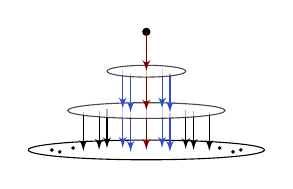
\begin{tikzpicture}[yscale=0.5]
      \node [circ] at (0, 3) {};

      \fill (1.2, 0) ellipse (0.025 and 0.05); % because yscale
      \fill (1.1, -0.05) ellipse (0.025 and 0.05);
      \fill (0.93, 0.05) ellipse (0.025 and 0.05);

      \fill (-1.2, 0) ellipse (0.025 and 0.05);
      \fill (-1.1, -0.05) ellipse (0.025 and 0.05);
      \fill (-0.93, 0.05) ellipse (0.025 and 0.05);

      \draw (0, 0) ellipse (1.5 and 0.25);

      \draw [-latex', mred] (0, 1) -- +(0, -1);
      \draw [-latex', mblue] (0.2, 1.05) -- +(0, -1);
      \draw [-latex', mblue] (0.3, 0.95) -- +(0, -1);
      \draw [-latex', mblue] (-0.3, 1.05) -- +(0, -1);
      \draw [-latex', mblue] (-0.2, 0.95) -- +(0, -1);

      \draw [-latex'] (0.5, 1.02) -- +(0, -1);
      \draw [-latex'] (0.8, 0.97) -- +(0, -1);
      \draw [-latex'] (0.6, 1) -- +(0, -1);
      \draw [-latex'] (-0.6, 1) -- +(0, -1);
      \draw [-latex'] (-0.5, 1.04) -- +(0, -1);
      \draw [-latex'] (-0.8, 0.97) -- +(0, -1);

      \draw [fill=white, opacity=0.7] (0, 1) ellipse (1 and 0.2);

      \draw [-latex', mred] (0, 2) -- +(0, -1);
      \draw [-latex', mblue] (0.2, 2.05) -- +(0, -1);
      \draw [-latex', mblue] (0.3, 1.95) -- +(0, -1);
      \draw [-latex', mblue] (-0.3, 2.05) -- +(0, -1);
      \draw [-latex', mblue] (-0.2, 1.95) -- +(0, -1);

      \draw [fill=white, opacity=0.7] (0, 2) ellipse (0.5 and 0.15);
      \draw [-latex', mred] (0, 3) -- +(0, -1);
    \end{tikzpicture}
  \end{center}

  Similarly, we can partition $X^{(\leq \lfloor n/2\rfloor)}$ into $m$ chains with each chain ending in $X^{(\lfloor n/2\rfloor)}$. Then glue them together.
\end{proof}

Another way to prove this result is to provide an alternative measure on how large an antichain can be, and this gives a stronger result.
\begin{thm}[LYM inequality]\index{LYM inequality}
  Let $\mathcal{A}$ be an antichain in $\mathcal{P}(X)$ with $|X| = n$. Then
  \[
    \sum_{r = 0}^n \frac{|\mathcal{A} \cap X^{(r)}|}{\binom{n}{r}} \leq 1.
  \]
  In particular, $|\mathcal{A}| \leq \max_r \binom{n}{r} = \binom{n}{\lfloor n/2\rfloor}$, as we already know.
\end{thm}

\begin{proof}
  A chain $C_0 \subseteq C_1 \subseteq \cdots \subseteq C_m$ is maximal if it has $n + 1$ elements. Moreover, there are $n!$ maximal chains, since we start with the empty set and then, given $C_i$, we produce $C_{i + 1}$ by picking one unused element and adding it to $C_i$.

  For every maximal chain $\mathcal{C}$, we have $|\mathcal{C} \cap \mathcal{A}| \leq 1$. Moreover, every set of $k$ elements appears in $k! (n - k)!$ maximal chains, by a similar counting argument as above. So
  \[
    \sum_{A \in \mathcal{A}} |A|! (n - |A|)! \leq n!.
  \]
  Then the result follows.
\end{proof}

There are analogous results for posets more general than just $\mathcal{P}(X)$. To formulate these results, we must introduce the following new terminology.
\begin{defi}[Shadow]\index{shadow}
  Given $A \subseteq S_i$, the \emph{shadow} at level $i - 1$ is
  \[
    \partial A = \{x \in S_{i - 1}: x < y\text{ for some }y \in A\}.
  \]
\end{defi}

\begin{defi}[Downward-expanding poset]\index{downward-expanding poset}
  A graded poset $P = (S, <)$ is said to be \emph{downward-expanding} if
  \[
    \frac{|\partial A|}{|S_{i - 1}|} \geq \frac{|A|}{|S_i|}
  \]
  for all $A \subseteq A_i$.

  We similarly define \term{upward-expanding}, and say a poset is \term{expanding} if it is upward or downward expanding.
\end{defi}

\begin{defi}[Weight]\index{weight}
  The \emph{weight} of a set $A \subseteq S$ is
  \[
    w(A) = \sum_{i = 0}^n \frac{|A \cap S_i|}{|S_i|}.
  \]
\end{defi}

The theorem is that the LYM inequality holds in general for any downward expanding posets.
\begin{thm}
  If $P$ is downward expanding and $A$ is an anti-chain, then $w(A) \leq 1$. In particular, $|A| \leq \max_i |S_i|$.

  Since each $S_i$ is an anti-chain, the largest anti-chain has size $\max_i |S_i|$.
\end{thm}

\begin{proof}
  We define the \emph{span} of $A$ to be
  \[
    \spn A = \max_{A_j \not= \emptyset} j - \min_{A_i \not= \emptyset} i.
  \]
  We do induction on $\spn A$.

  If $\spn A = 0$, then we are done. Otherwise, let $h_i = \max_{A_j \not= 0} j$, and set $B_{h - 1} = \partial A_h$. Then since $A$ is an anti-chain, we know $A_{h - 1} \cap B_{h - 1} = \emptyset$.

  We set $A' = A \setminus A_h \cup B_{h - 1}$. This is then another anti-chain, by the transitivity of $<$. We then have
  \[
    w(A) = w(A') + w(A_h) - w(B_{h - 1}) \leq w(A') \leq 1,
  \]
  where the first inequality uses the downward-expanding hypothesis and the second is the induction hypothesis.
\end{proof}

We may want to mimic our other proof of the fact that the largest size of an antichain in $\mathcal{P}(X)$ is $\binom{n}{\lfloor n/2\rfloor}$. This requires the notion of a \emph{regular poset}.

\begin{defi}[Regular poset]\index{regular poset}\index{poset!regular}
  We say a graded poset $(S, <)$ is \emph{regular} if for each $i$, there exists $r_i, s_i$ such that if $x \in A_i$, then $x$ dominates $r_i$ elements at level $i - 1$, and is dominated by $s_i$ elements at level $i + 1$.
\end{defi}
%We observe that being regular implies being expanding.
%Note that being regular implies being expanding. So we know

\begin{prop}
  An anti-chain in a regular poset has weight $\leq 1$.
\end{prop}

\begin{proof}
  Let $M$ be the number of maximal chains of length $(n + 1)$, and for each $x \in S_k$, let $m(x)$ be the number of maximal chains through $x$. Then
  \[
    m(x) = \prod_{i = 1}^k r_i \prod_{i = k}^{n - 1} s_i.
  \]
  So if $x, y \in S_i$, then $m(x) = m(y)$.

  Now since every maximal chain passes through a unique element in $S_i$, for each $x \in S_i$, we have
  \[
    M = \sum_{x \in S_i} m(x) = |S_i| m(x).
  \]
  This gives the formula
  \[
    m(x) = \frac{M}{|S_i|}.
  \]
  now let $A$ be an anti-chain. Then $A$ meets each chain in $\leq 1$ elements. So we have
  \[
    M = \sum_{\text{maximal chains}} 1 \geq \sum_{x \in A} m(x) = \sum_{i = 0}^n |A \cap S_i| \cdot \frac{M}{|S_i|}.
  \]
  So it follows that
  \[
    \sum \frac{|A \cap S_i|}{|S_i|} \leq 1.\qedhere
  \]
\end{proof}

%\subsection{Littlewood--Offord problem}
%In the 1930s and 1940s, people were studying roots of random polynomials of the form
%\[
%  \sum_{k = 0}^n \varepsilon_k x^k,
%\]
%where $\varepsilon_k = 0, 1$.

Let's now turn to a different problem. Suppose $x_1, \ldots, x_n \in \C$, with each $|x_i| \geq 1$. Given $A \subseteq [n]$, we let
\[
  x_A = \sum_{i \in A} x_i.
\]
We now seek the largest size of $\mathcal{A}$ such that $|x_A - x_B| < 1$ for all $A, B \in \mathcal{A}$. More precisely, we want to find the best choice of $x_1, \ldots, x_n$ and $\mathcal{A}$ so that $|\mathcal{A}|$ is as large as possible while satisfying the above condition.

If we are really lazy, then we might just choose $x_i = 1$ for all $i$. By taking $\mathcal{A} = [n]^{\lfloor n/2\rfloor}$, we can obtain $|\mathcal{A}| = \binom{n}{\lfloor n/2\rfloor}$.

Erd\"os noticed this is the best bound if we require the $x_i$ to be real.

\begin{thm}[Erd\"os, 1945]
  Let $x_i$ be all real, $|x_i| \geq 1$. For $A \subseteq [n]$, let
  \[
    x_A = \sum_{i \in A} x_i.
  \]
  Let $\mathcal{A} \subseteq \mathcal{P}(n)$. Then $|\mathcal{A}| \leq \binom{n}{\lfloor n/2\rfloor}$.
\end{thm}

\begin{proof}
  We claim that we may assume $x_i \geq 1$ for all $i$. To see this, suppose we instead had $x_1 = -2$, say. Then whether or not $i \in A$ determines whether $x_A$ should include $0$ or $-2$ in the sum. If we replace $x_i$ with $2$, then whether or not $i \in A$ determines whether $x_A$ should include $0$ or $2$. So replacing $x_i$ with $2$ just essentially shifts all terms by $2$, which doesn't affect the difference.

  But if we assume that $x_i \geq 1$ for all $i$, then we are done, since $\mathcal{A}$ must be an anti-chain, for if $A, B \in \mathcal{A}$ and $A \subsetneq B$, then $x_B - x_A = x_{B\setminus A} \geq 1$.
\end{proof}

Doing it for complex numbers is considerably harder. In 1970, Kleitman found a gorgeous proof for \emph{every} normed space. This involves the notion of a \emph{symmetric decomposition}. To motivate this, we first consider the notion of a symmetric chain.

\begin{defi}[Symmetric chain]\index{symmetric chain}
  We say a chain $\mathcal{C} = \{C_i, C_{i + 1}, \ldots, C_{n - i}\}$ is \emph{symmetric} if $|C_j| = j$ for all $j$.
\end{defi}

\begin{thm}
  $\mathcal{P}(n)$ has a decomposition into symmetric chain.
\end{thm}

\begin{proof}
  We prove by induction. In the case $n = 1$, we simply have to take $\{\emptyset, \{1\}\}$.

  Now suppose $\mathcal{P}(n- 1)$ has a symmetric chain decomposition $\mathcal{C}_1 \cup \cdots \cup \mathcal{C}_t$. Given a symmetric chain
  \[
    \mathcal{C}_j = \{C_i, C_{i + 1}, \ldots, C_{n - 1 - i}\},
  \]
  we obtain two chains $\mathcal{C}_j^{(0)}, \mathcal{C}_j^{(1)}$ in $\mathcal{P}(n)$ by
  \begin{align*}
    \mathcal{C}_j^{(0)} &= \{C_i, C_{i + 1}, \ldots, C_{n - 1 - i}, C_{n - 1 - i} \cup \{n\}\}\\
    \mathcal{C}_j^{(1)} &= \{C_i \cup\{n\}, C_{i + 1} \cup \{n\}, \ldots, C_{n - 2 - i} \cup \{n\}\}.
  \end{align*}
  Note that if $|\mathcal{C}_j| = 1$, then $\mathcal{C}_j^{(1)} = \emptyset$, and we drop this. Under this convention, we note that every $A \in \mathcal{P}(n)$ appears in exactly one $\mathcal{C}_j^{(\varepsilon)}$, and so we are done.
\end{proof}

We are not going to actually need the notion of symmetric chains in our proof. What we need is the ``profile'' of a symmetric chain decomposition. By a simple counting argument, we see that for $0 \leq i \leq \frac{n}{2}$, the number of chains with $n + 1 - 2i$ sets is
\[
  \ell(n, i) \equiv \binom{n}{i} - \binom{n}{i - 1}.
\]
\begin{thm}[Kleitman, 1970]
  Let $x_1, x_2, \ldots, x_n$ be vectors in a normed space with norm $\|x_I\| \geq 1$ for all $i$. For $A \in \mathcal{P}(n)$, we set
  \[
    x_A = \sum_{i \in A} x_i.
  \]
  Let $\mathcal{A} \subseteq \mathcal{P}(n)$ be such that $\|x_A - x_B\|< 1$. Then $\|\mathcal{A}\| \leq \binom{n}{\lfloor n/2\rfloor}$.
\end{thm}
This bound is indeed the best, since we can pick $x_i = x$ for some $\|x\| \geq 1$, and then we can pick $\mathcal{A} = [n]^{\lfloor n/2\rfloor}$.

\begin{proof}
  Call $\mathcal{F} \subseteq \mathcal{P}(n)$ \emph{sparse} if $\|x_E - x_F\| \geq 1$ for all $E, F \in \mathcal{F}$, $E \not= F$. Note that if $\mathcal{F}$ is sparse, then $|\mathcal{F} \cap \mathcal{A}| \leq 1$. So if we can find a decomposition of $\mathcal{P}(n)$ into $\binom{n}{\lfloor n/2\rfloor}$ sparse sets, then we are done.

  We call a partition $\mathcal{P}(n) = \mathcal{F}_1 \cup \cdots \cup F_t$ \emph{symmetric} if the number of families with $n + 1 - 2i$ sets is $\ell(n, i)$, i.e.\ the ``profile'' is that of a symmetric chain decomposition.

  \begin{claim}
    $\mathcal{P}(n)$ has a symmetric decomposition into sparse families.
  \end{claim}

  We again induct on $n$. When $n = 1$, we can take $\{\emptyset, \{1\}\}$. Now suppose $\Delta_{n - 1}$ is a symmetric decomposition of $\mathcal{P}(n - 1)$ as $\mathcal{F}_1 \cup \cdots \cup \mathcal{F}_t$.

  Given $\mathcal{F}_j$, we construct $\mathcal{F}_j^{(0)}$ and $\mathcal{F}_j^{(1)}$ ``as before''. We pick some $D \in \mathcal{F}_j$, to be decided later, and we take
  \begin{align*}
    \mathcal{F}_j^{(0)} &= \mathcal{F}_j \cup\{ D \cup \{n\}\}\\
    \mathcal{F}_j^{(1)} &= \{ E \cup \{n\}: E \in \mathcal{F}_j \setminus \{D\}\}.
  \end{align*}
  The resulting set is certainly still symmetric. The question is whether it is sparse, and this is where the choice of $D$ comes in. The collection $\mathcal{F}_j^{(1)}$ is certainly still sparse, and we must pick a $D$ such that $\mathcal{F}_j^{(0)}$ is sparse.

  To do so, we use Hahn--Banach to obtain a linear functional $f$ such that $\|f\| = 1$ and $f(x_n) = \|x_n\| \geq 1$. We can then pick $D$ to maximize $f(x_D)$. Then we check that if $E \in \mathcal{F}_j$, then
  \[
    f(x_{D \cup \{n\}} - x_2) = f(x_D) - f(x_E) + f(x_n).
  \]
  By assumption, $f(x_n) \geq 1$ and $f(x_D) \geq f(x_E)$. So this is $\geq 1$. Since $\|f\| = 1$, it follows that $\|x_{D \cup \{n\}} - x_E\| \geq 1$.
\end{proof}

\section{The Kruskal--Katona theorem}
For $\mathcal{A} \subseteq X^{(r)}$, recall we defined the lower shadow to be
\[
  \partial \mathcal{A} = \{B \in X^{(r - 1)} : B \subseteq A \text{ for some } A \in \mathcal{A}\}.
\]
The question we wish to understand is how small we can make $\partial \mathcal{A}$, relative to $\mathcal{A}$. Crudely, we can bound the size by
\[
  |\partial \mathcal{A}| \geq |\mathcal{A}| \frac{\binom{n}{r - 1}}{\binom{n}{r}} = \frac{n - r}{r} |\mathcal{A}|.
\]
But surely we can do better than this. To do so, one reasonable strategy is to first produce some choice of $\mathcal{A}$ we think is optimal, and see how we can prove that it is indeed optimal.

To do so, let's look at some examples.
\begin{eg}
  Take $n = 6$ and $r = 3$. We pick
  \[
    \mathcal{A} = \{123, 456, 124, 256\}.
  \]
  Then we have
  \[
    \partial \mathcal{A} = \{12, 13, 23, 45, 46, 56, 14, 24, 25, 26\},
  \]
  and this has $10$ elements.

  But if we instead had
  \[
    \mathcal{A} = \{123, 124, 134, 234\},
  \]
  then
  \[
    \partial \mathcal{A} = \{12, 13, 14, 23, 24, 34\},
  \]
  and this only has $6$ elements, and this is much better.
\end{eg}
Intuitively, the second choice of $\mathcal{A}$ is better because the terms are ``bunched'' together.

More generally, we would expect that if we have $|\mathcal{A}| = \binom{k}{r}$, then the best choice should be $\mathcal{A} = [k]^{(r)}$, with $|\partial A| = \binom{k}{r - 1}$. For other choices of $\mathcal{A}$, perhaps a reasonable strategy is to find the largest $k$ such that $\binom{k}{r} < |\mathcal{A}|$, and then take $\mathcal{A}$ to be $[k]^{(r)}$ plus some elements. To give a concrete description of which extra elements to pick, our strategy is to define a total order on $[n]^{(r)}$, and say we should pick the initial segment of length $|\mathcal{A}|$.

This suggests the following proof strategy:
\begin{enumerate}
  \item Come up with a total order on $[n]^{(r)}$, or even $\N^{(r)}$ such that $[k]^{(r)}$ are initial segments for all $k$.
  \item Construct some ``compression'' operators\index{compression operator} $\mathcal{P}(\N^{(r)}) \to \mathcal{P}(\N^{(r)})$ that pushes each element down the ordering without increasing the $|\partial \mathcal{A}|$.
  \item Show that the only subsets of $\N^{(r)}$ that are fixed by the compression operators are the initial segments.
\end{enumerate}
There are two natural orders one can put on $[n]^{(r)}$:
\begin{itemize}
  \item lex\index{lex order}: We say $A < B$ if $\min A \Delta B \in A$.
  \item colex\index{colex order}: We say $A < B$ if $\max A \Delta B \in B$.
\end{itemize}
\begin{eg}
  For $r = 3$, the elements of $X^{(3)}$ in colex order are
  \[
    123, 124, 134, 234, 125, 135, 235, 145, 245, 345, 126,\ldots
  \]
\end{eg}

In fact, colex is an order on $\N^{(r)}$, and we see that the initial segment with $\binom{n}{r}$ elements is exactly $[n]^{(r)}$. So this is a good start.

If we believe that colex is indeed the right order to do, then we ought to construct some compression operators. For $i \not= j$, we define the $(i, j)$-compression as follows: for a set $A \in X^{(r)}$, we define
\[
  C_{ij}(A) =
  \begin{cases}
    (A \setminus \{j\}) \cup \{i\} & j \in A, i \not\in A\\
    A & \text{otherwise}
  \end{cases}
\]
For a set system, we define
\[
  C_{ij}(\mathcal{A}) = \{C_{ij}(A): A \in \mathcal{A}\} \cup \{A \in \mathcal{A}:C_{ij}(A) \in \mathcal{A}\}
\]
We can picture our universe of sets as follows:
\begin{center}
  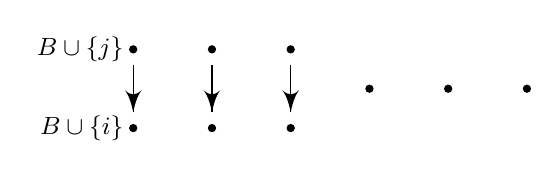
\begin{tikzpicture}
    \foreach \x in {0,1,2} {
      \node [circ] at (\x, 0) {};
      \node [circ] at (\x, -1) {};
      \draw [->] (\x, -0.2) -- (\x, -0.8) {};
    }
    \node [left] at (0, 0) {\small$B \cup \{j\}$};
    \node [left] at (0, -1) {\small$B \cup \{i\}$};
    \foreach \y in {3, 4, 5} {
      \node [circ] at (\y, -0.5) {};
    }
  \end{tikzpicture}
\end{center}
The set system $\mathcal{A}$ is some subset of all these points, and we what we are doing is that we are pushing everything down when possible.

It is clear that we have $|C_{ij}(\mathcal{A})| = |\mathcal{A}|$. We further observe that

\begin{lemma}
  We have
  \[
    \partial C_{ij}(\mathcal{A}) \subseteq C_{ij}(\partial \mathcal{A}).
  \]
  In particular, $|\partial C_{ij}(\mathcal{A})| \leq |\partial \mathcal{A}|$.\qedsym
\end{lemma}

Given $\mathcal{A} \subseteq X^{(r)}$, we say $\mathcal{A}$ is left-compressed if $c_{ij}(\mathcal{A}) = \mathcal{A}$ for all $i < j$. Is this good enough?

Of course initial segments are left-compressed. However, it turns out the converse is not true.

\begin{eg}
  $\{123, 124, 125, 126\}$ are left-compressed, but not an initial segment.
\end{eg}

So we want to come up with ``more powerful'' compressions. For $U, V \in X^{(s)}$ with $U \cap V = \emptyset$, we define a $(U, V)$-compression as follows: for $A \subseteq X$, we define
\[
  C_{UV}(A) =
  \begin{cases}
    (A \setminus V) \cup U & A \cap (U \cup V) = V\\
    A & \text{otherwise}
  \end{cases}
\]
Again, for $\mathcal{A} \subseteq X^{(r)}$, we can define
\[
  C_{UV}(\mathcal{A}) = \{C_{UV}(A) : A \in \mathcal{A}\} \cup \{A \in \mathcal{A}: C_{UV}(A) \in \mathcal{A}\}.
\]
Again, $\mathcal{A}$ is $(U, V)$-compressed if $C_{UV}(\mathcal{A}) = \mathcal{A}$.

This time the behaviour of the compression is more delicate.
\begin{lemma}
  Let $\mathcal{A} \subseteq X^{(r)}$ and $U, V \in X^{(s)}$, $U \cap V = \emptyset$. Suppose for all $u \in U$, there exists $v$ such that $\mathcal{A}$ is $(U \setminus \{u\}, V \setminus \{v\})$-compressed. Then
  \[
    \partial C_{UV} (\mathcal{A}) \subseteq C_{UV}(\partial A).\tag*{$\square$}
  \]
\end{lemma}

\begin{lemma}
  $\mathcal{A} \subseteq X^{(r)}$ is an initial segment of $X^{(r)}$ in colex if and only if it is $(U, V)$-compressed for all $U, V$ disjoint with $|U| = |V|$ and $\max V > \max U$.
\end{lemma}

\begin{proof}
  $\Rightarrow$ is clear. Suppose $\mathcal{A}$ is $(U, V)$ compressed for all such $U, V$. If $\mathcal{A}$ is not an initial segment, then there exists $B \in \mathcal{A}$ and $C \not \in \mathcal{A}$ such that $C < B$. Then $\mathcal{A}$ is not $(C \setminus B, B \setminus C)$-compressed. A contradiction.
\end{proof}

\begin{lemma}
  Given $\mathcal{A} \in X^{(r)}$, there exists $\mathcal{B} \subseteq X^{(r)}$ such that $\mathcal{B}$ is $(U, V)$-compressed for all $|U| = |V|$, $U \cap V= \emptyset$, $\max V > \max U$, and moreover
  \[
    |\mathcal{B}| = |\mathcal{A}|, |\partial \mathcal{B}| \leq |\partial \mathcal{A}|.\tag{$*$}
  \]
\end{lemma}

\begin{proof}
  Let $\mathcal{B}$ be such that
  \[
    \sum_{B \in \mathcal{B}} \sum_{i \in B} 2^i
  \]
  is minimal among those $\mathcal{B}$'s that satisfy $(*)$. We claim that this $\mathcal{B}$ will do. Indeed, if there exists $(U, V)$ such that $|U| = |V|$, $\max V > \max U$ and $C_{UV}(\mathcal{B}) \not= \mathcal{B}$, then pick such a pair with $|U|$ minimal. Then apply a $(U, V)$-compression, which is valid since given any $u \in U$ we can pick any $v \in V$ that is not $\max V$ to satisfy the requirements of the previous lemma. This decreases the sum, which is a contradiction.
\end{proof}

From these, we conclude that
\begin{thm}[Kruskal 1963, Katona 1968]
  Let $\mathcal{A} \subseteq X^{(r)}$, and let $\mathcal{C} \subseteq X^{(r)}$ be the initial segment with $|\mathcal{C}| = |\mathcal{A}|$. Then
  \[
    |\partial \mathcal{A}| \geq |\partial \mathcal{C}|.
  \]
\end{thm}

We can now define the \term{shadow function}
\[
  \partial^{(r)}(m) = \min\{|\partial \mathcal{A}| : \mathcal{A} \subseteq X^{(r)}, |\mathcal{A}| = m\}.
\]
This does not depend on the size of $X$ as long as $X$ is large enough to accommodate $m$ sets, i.e.\ $\binom{n}{r} \geq m$. It would be nice if we can concretely understand this function. So let's try to produce some initial segments.

Essentially by definition, an initial segment is uniquely determined by the last element. So let's look at some examples.
\begin{eg}
  Take $r = 4$. What is the size of the initial segment ending in $3479$? We note that anything that ends in something less than $8$ is less that $3479$, and there are $\binom{8}{4}$ such elements. If you end in $9$, then you are still fine if the second-to-last digit is less than $7$, and there are $\binom{6}{3}$ such elements. Continuing, we find that there are
  \[
    \binom{8}{4} + \binom{6}{3} + \binom{4}{2}
  \]
  such elements.
\end{eg}

Given $m_r > m_{r - 1} > \cdots > m_s \geq s$, we let$\mathcal{B}^{(r)}(m_r, m_{r - 1}, \ldots, m_s)$ be the initial segment ending in the element
\[
  m_r + 1, m_{r - 1} + 1, \ldots, m_{s + 1} + 1, m_s, m_s - 1, m_s - 2, \ldots, m_s - (s - 1).
\]
This consists of the sets $\{a_1 < a_2 < \cdots < a_r\}$ such that there exists $j \in [s, r]$ with $a_i = m_i + 1$ for $i > j$, and $a_j \leq m_j$.

To construct an element in $\mathcal{B}^{(r)}(m_r, \ldots, m_s)$, we need to first pick a $j$, and then select $j$ elements that are $\leq m_j$. Thus, we find that
\[
  |\mathcal{B}^{(r)}(m_r, \ldots, m_s)| = \sum_{j = s}^r \binom{m_j}{j} = b^{(r)} (m_1, \ldots, m_s).
\]
We see that this $\mathcal{B}^{(r)}$ is indeed the initial segment in the colex order ending in that element. So we know that for all $m \in \N$, there is a unique sequence $m_r > m_{r - 1} > \ldots, > m_s \geq s$ such that $n = \sum_{j = 0}^r \binom{m_j}{j}$.

It is also not difficult to find the shadow of this set. After a bit of thinking, we see that it is given by
\[
  \mathcal{B}^{(r - 1)} (m_r, \ldots, m_s).
\]
Thus, we find that
\[
  \partial^{(r)}\left( \sum_{i = s}^r \binom{m_i}{i}\right) = \sum_{i = s}^r \binom{m_i}{i - 1},
\]
and moreover every $m$ can be expressed in the form $\sum_{i = s}^r \binom{m_i}{i}$ for some unique choices of $m_i$.

In particular, we have
\[
  \partial^{(r)}\left(\binom{n}{r}\right) = \binom{n}{r - 1}.
\]
Since it might be slightly annoying to write $m$ in the form $\sum_{i = s}^r \binom{m_i}{i}$, Lov\'asz provided another slightly more convenient bound.
\begin{thm}[Lov\'asz, 1979]
  If $\mathcal{A} \subseteq X^{(r)}$ with $|\mathcal{A}| = \binom{x}{r}$ for $x \geq 1, x \in \R$, then
  \[
    |\partial \mathcal{A}| \geq \binom{x}{r - 1}.
  \]
  This is best possible if $x$ is an integer.
\end{thm}

\begin{proof}
  Let
  \begin{align*}
    \mathcal{A}_0 &= \{A \in \mathcal{A}: 1 \not \in A\}\\
    \mathcal{A}_1 &= \{A \in \mathcal{A}: 1 \in A\}.
  \end{align*}
  For convenience, we write
  \[
    \mathcal{A}_1 - 1 = \{A \setminus \{1\}: A \in \mathcal{A}_1\}.
  \]
  We may assume $\mathcal{A}$ is $(i, j)$-compressed for all $i < j$. We induct on $r$ and then on $|\mathcal{A}|$. We have
  \[
    |\mathcal{A}_0| = |\mathcal{A}| - |\mathcal{A}_1|.
  \]
  We note that $\mathcal{A}_1$ is non-empty, as $\mathcal{A}$ is left-compressed. So $|\mathcal{A}_0| < |\mathcal{A}|$.

  If $r = 1$ and $|\mathcal{A}| = 1$ then there is nothing to do.

  Now observe that $\partial \mathcal{A} \subseteq \mathcal{A}_1 - 1$, since if $A \in \mathcal{A}$, $1 \not \in A$, and $B \subseteq A$ is such that $|A \setminus B| = 1$, then $B \cup \{1\} \in \mathcal{A}_1$ since $\mathcal{A}$ is left-compressed. So it follows that
  \[
    |\partial \mathcal{A}_0| \leq |\mathcal{A}_1|.
  \]
  Suppose $|\mathcal{A}_1| < \binom{x - 1}{r - 1}$. Then
  \[
    |\mathcal{A}_0| > \binom{x}{r} - \binom{x - 1}{r - 1} = \binom{x - 1}{r}.
  \]
  Therefore by induction, we have
  \[
    |\partial \mathcal{A}_0| > \binom{x - 1}{r - 1}.
  \]
  This is a contradiction, since $|\partial \mathcal{A}_0| \leq |\mathcal{A}_1|$. Hence $|\mathcal{A}_1| \geq \binom{x - 1}{r - 1}$. Hence we are done, since
  \[
    |\partial \mathcal{A}| \geq |\partial \mathcal{A}_1| = |\mathcal{A}_1| + |\partial (\mathcal{A}_1 - 1)| \geq \binom{x - 1}{r - 1} + \binom{x - 1}{r - 2} = \binom{x}{r - 1}.\qedhere
  \]
\end{proof}

%$r = 2$ is a non-starter. Given $m$ edges on $[n]$, at least how many vertices do they have altogether? If $m > \binom{k}{2}$, then $|\mathrm{shadow}| \geq k + 1$. Thus, if
%\[
%  \binom{k - 1}{2} < m \leq \binom{k}{2},
%\]
%then for
%\[
%  \mathcal{A} \subseteq X^{(2)} = [n]^{(2)}
%\]
%with $|\mathcal{A}| = m$, then $|\partial A| \geq k$. This is the best possible.
%
%We hope that if $\mathcal{A} \subseteq X^{(r)}$ and $\mathcal{C}$ is the initial segment of $X^{(r)}$ in colex with $|\mathcal{C}| = |\mathcal{A}|$, then
%\[
%  |\partial \mathcal{A}| \geq |\partial \mathcal{C}|.
%\]
%
%

\section{Isoperimetric inequalities}
We are now going to ask a question similar to the one answered by Kruskal--Katona. Kruskal--Katona answered the question of how small can $\partial \mathcal{A}$ be among all $\mathcal{A} \subseteq X^{(r)}$ of fixed size. Clearly, we obtain the same answer if we sought to minimized the upper shadow instead of the lower. But what happens if we want to minimize both the upper shadow and the lower shadow? Or, more generally, if we allow $\mathcal{A} \subseteq \mathcal{P}(X)$ to contain sets of different sizes, how small can the set of ``neighbours'' of $\mathcal{A}$ be?

\begin{defi}[Boundary]\index{boundary}
  Let $G$ be a graph and $A \subseteq V(A)$. Then the \emph{boundary} $b(A)$ is the set of all $x \in G$ such that $x \not \in A$ but $x$ is adjacent to $A$.
\end{defi}

\begin{eg}
  In the following graph
  \begin{center}
    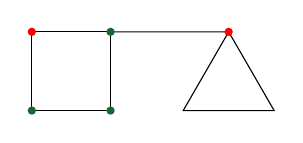
\begin{tikzpicture}

      \draw (0, 0) rectangle (1, 1);
      \draw (1, 1) -- (2.5, 1) -- (3.07736, 0) -- (1.92264, 0) -- (2.5, 1);

      \node [circ, mgreen] at (0, 0) {};
      \node [circ, mgreen] at (1, 0) {};
      \node [circ, mgreen] at (1, 1) {};
      \node [circ, red] at (0, 1) {};
      \node [circ, red] (a) at (2.5, 1) {};

    \end{tikzpicture}
  \end{center}
  the boundary of the green vertices is the red vertices.
\end{eg}

An \term{isoperimetric inequality} on $G$ is an inequality of the form
\[
  |b(A)| \geq f(|A|)
\]
for all $A \subseteq G$. Of course, we could set $f \equiv 0$, but we would like to do better than that.

The ``continuous version'' of this problem is well-known. For example, in a plane, given a fixed area, the perimeter of the area is minimized if we pick the area to be a disc. Similarly, among subsets of $\R^3$ of a given volume, the solid sphere has the smallest surface area. Slightly more exotically, among subsets of $S^2$ of given area, the circular cap has smallest perimeter.

Before we proceed, we note the definition of a \emph{neighbourhood}:
\begin{defi}[Neighbourhood]\index{neighbourhood}
  Let $G$ be a graph and $A \subseteq V(A)$. Then the \emph{neighbourhood} of $A$ is $N(A) = A \cup b(A)$.
\end{defi}
Of course, $|b(A)| = |N(A)| - |A|$, and it is often convenient to express and prove our isoperimetric inequalities in terms of the neighbourhood instead.

If we look at our continuous cases, then we observe that all our optimal figures are balls, i.e.\ they consist of all the points a distance at most $r$ from a point, for some $r$ and single point. We would hope that this pattern generalizes.

Of course, it would be a bit ambitious to hope that balls are optimal for all graphs. However, we can at least show that it is true for the graphs we care about, namely graphs obtained from power sets.

\begin{defi}[Discrete cube]\index{discrete cube}
  Given a set $X$, we turn $\P(X)$ into a graph as follows: join $x$ to $y$ if $|x \Delta y| = 1$, i.e.\ if $x = y \cup \{a\}$ for some $a \not \in y$, or vice versa.

  This is the \emph{discrete cube} $Q_n$, where $n = |X|$.
\end{defi}

\begin{eg}
  $Q_3$ looks like
  \begin{center}
    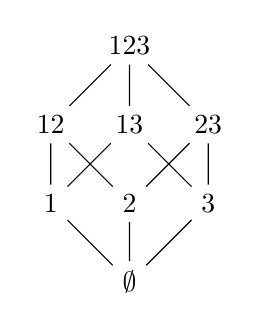
\begin{tikzpicture}
      \node (123) at (0, 0) {123};

      \node (13) at (0, -1) {13};
      \node (12) at (-1, -1) {12};
      \node (23) at (1, -1) {23};

      \node (2) at (0, -2) {2};
      \node (1) at (-1, -2) {1};
      \node (3) at (1, -2) {3};

      \node (0) at (0, -3) {$\emptyset$};

      \draw (0) -- (1) -- (12) -- (123);
      \draw (0) -- (3) -- (23) -- (123);
      \draw (0) -- (2) -- (12);
      \draw (2) -- (23);
      \draw (1) -- (13) -- (123);
      \draw (3) -- (13);
    \end{tikzpicture}
  \end{center}
\end{eg}
This looks like a cube! Indeed, if we identify each $x \in \Q$ with the 0-1 sequence of length $n$ (e.g.\ $13 \mapsto 101000\cdots 0$), or, in other words, its indicator function, then $Q_n$ is naturally identified with the unit cube in $\R^n$.
\begin{center}
  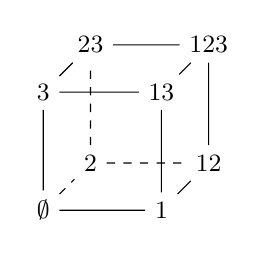
\begin{tikzpicture}[scale=1.5]
    \node (0) at (0, 0) {\small$\emptyset$};
    \node (1) at (1, 0) {\small$1$};
    \node (3) at (0, 1) {\small$3$};
    \node (2) at (0.4, 0.4) {\small$2$};
    \node (12) at (1.4, 0.4) {\small$12$};
    \node (13) at (1, 1) {\small$13$};
    \node (23) at (0.4, 1.4) {\small$23$};
    \node (123) at (1.4, 1.4) {\small$123$};

    \draw (0) -- (1) -- (12) -- (123) -- (23) -- (3) -- (0);
    \draw (3) -- (13) -- (1);
    \draw (13) -- (123);

    \draw [dashed] (0) -- (2) -- (12);
    \draw [dashed] (2) -- (23);

  \end{tikzpicture}
\end{center}
Note that in this picture, the topmost layer is the points that do have $3$, and the bottom layer consists of those that do not have a $3$, and we can make similar statements for the other directions.

\begin{eg}
  Take $Q_3$, and try to find a size $A$ of size $4$ that has minimum boundary. There are two things we might try --- we can take a slice, or we can take a ball. In this case, we see the ball is the best.
\end{eg}
We can do more examples, and it appears that the ball $X^{(\leq r)}$ is the best all the time. So that might be a reasonable thing to try to prove. But what if we have $|A|$ such that $|X^{(\leq r)}| < |A| < |X^{(\leq r + 1)}$?

It is natural to think that we should pick an $A$ with $X^{(\leq r)} \subseteq A \subseteq X^{(\leq r + 1)}$, so we set $A = X^{(\leq r)} \cup B$, where $B \subseteq X^{(r + 1)}$. Such an $A$ is known as a \term{Hamming ball}\index{ball!Hamming}.

What $B$ should we pick? Observe that
\[
  N(A) = X^{(\leq r + 1)} \cup \partial^+ B.
\]
So we want to pick $B$ to minimize the \emph{upper} shadow. So by Kruskal--Katona, we know we should pick $B$ to be the initial segment in the lex order.

Thus, if we are told to pick $1000$ points to minimize the boundary, we go up in levels, and in each level, we go up in lex.
\begin{defi}[Simplicial ordering]\index{simplicial ordering}
  The \emph{simplicial ordering} on $Q_n$ is defined by $x < y$ if either $|x| < |y|$, or $|x| = |y|$ and $x < y$ in lex.
\end{defi}
Our aim is to show that the initial segments of the simplicial order minimize the neighbourhood. Similar to Kruskal--Katona, a reasonable strategy would be to prove it by compression.

For $A \subseteq Q_n$, and $1 \leq i \leq n$, the $i$-sections of $A$ are $A_+^{(i)}, A_-^{(i)} \subseteq \P(X\setminus \{i\})$ defined by
\begin{align*}
  A_-^{(i)} &= \{x \in A: i \not\in x\}\\
  A_+^{(i)} &= \{x \setminus \{i\}: x \in A, i \in x\}.
\end{align*}
These are the top and bottom layers in the $i$ direction.

The $i$-compression (or \term{co-dimension $1$ compression}) of $A$ is $C_i(A)$, defined by
\begin{align*}
  C_i(A)_+ &= \text{first $|A_+|$ elements of $\P(X \setminus \{i\})$ in simplicial}\\
  C_i(A)_- &= \text{first $|A_-|$ elements of $\P(X \setminus \{i\})$ in simplicial}
\end{align*}

\begin{eg}
  Suppose we work in $Q_4$, where the original set is
  \begin{center}
    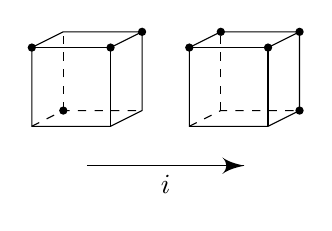
\begin{tikzpicture}
      \draw (0, 0) -- (1, 0) -- (1.4, 0.2) -- (1.4, 1.2) -- (0.4, 1.2) -- (0, 1) -- cycle;
      \draw (0, 1) -- (1, 1) -- (1, 0);
      \draw (1, 1) -- (1.4, 1.2);
      \draw [dashed] (0, 0) -- (0.4, 0.2) -- (1.4, 0.2);
      \draw [dashed] (0.4, 0.2) -- (0.4, 1.2);

      \node [circ] at (0.4, 0.2) {};
      \node [circ] at (0, 1) {};
      \node [circ] at (1, 1) {};
      \node [circ] at (1.4, 1.2) {};
      \begin{scope}[shift={(2, 0)}]
        \draw (0, 0) -- (1, 0) -- (1.4, 0.2) -- (1.4, 1.2) -- (0.4, 1.2) -- (0, 1) -- cycle;
        \draw (0, 1) -- (1, 1) -- (1, 0);
        \draw (1, 1) -- (1.4, 1.2);
        \draw [dashed] (0, 0) -- (0.4, 0.2) -- (1.4, 0.2);
        \draw [dashed] (0.4, 0.2) -- (0.4, 1.2);

        \node [circ] at (1, 1) {};
        \node [circ] at (0, 1) {};
        \node [circ] at (0.4, 1.2) {};
        \node [circ] at (1.4, 1.2) {};
        \node [circ] at (1.4, 0.2) {};
      \end{scope}

      \draw [->] (0.7, -0.5) -- (2.7, -0.5) node [pos=0.5, below] {$i$};
    \end{tikzpicture}
  \end{center}
  The resulting set is then
  \begin{center}
    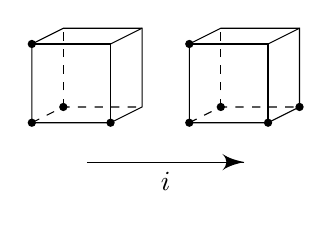
\begin{tikzpicture}
      \draw (0, 0) -- (1, 0) -- (1.4, 0.2) -- (1.4, 1.2) -- (0.4, 1.2) -- (0, 1) -- cycle;
      \draw (0, 1) -- (1, 1) -- (1, 0);
      \draw (1, 1) -- (1.4, 1.2);
      \draw [dashed] (0, 0) -- (0.4, 0.2) -- (1.4, 0.2);
      \draw [dashed] (0.4, 0.2) -- (0.4, 1.2);

      \node [circ] at (0, 0) {};
      \node [circ] at (0, 1) {};
      \node [circ] at (1, 0) {};
      \node [circ] at (0.4, 0.2) {};
      \begin{scope}[shift={(2, 0)}]
        \draw (0, 0) -- (1, 0) -- (1.4, 0.2) -- (1.4, 1.2) -- (0.4, 1.2) -- (0, 1) -- cycle;
        \draw (0, 1) -- (1, 1) -- (1, 0);
        \draw (1, 1) -- (1.4, 1.2);
        \draw [dashed] (0, 0) -- (0.4, 0.2) -- (1.4, 0.2);
        \draw [dashed] (0.4, 0.2) -- (0.4, 1.2);

        \node [circ] at (0, 0) {};
        \node [circ] at (0, 1) {};
        \node [circ] at (1, 0) {};
        \node [circ] at (0.4, 0.2) {};
        \node [circ] at (1.4, 0.2) {};
      \end{scope}

      \draw [->] (0.7, -0.5) -- (2.7, -0.5) node [pos=0.5, below] {$i$};
    \end{tikzpicture}
  \end{center}
\end{eg}
Clearly, we have $|C_i(A)| = |A|$, and $C_i(A)$ ``looks more like'' an initial segment in simplicial ordering than $A$ did.

We say $A$ is \emph{$i$-compressed} if $C_i(A) = A$.

\begin{lemma}
  For $A \subseteq Q_n$, we have $|N(C_i(A))| \leq |N(A)|$.
\end{lemma}

\begin{proof}
  We have
  \[
    |N(A)| = |N(A_+) \cup A_-| + |N(A_-) \cup A_+|
  \]
  Take $B = C_i(A)$. Then
  \begin{align*}
    |N(B)| &= |N(B_+) \cup B_-| + |N(B_-) \cup B_+|\\
    &= \max \{|N(B_+)|, |B_-|\} + \max \{|N(B_-)|, |B_+|\}\\
    &\leq \max \{|N(A_+)|, |A_-|\} + \max \{|N(A_-)|, |A_+|\}\\
    &\leq |N(A_+) \cup A_i| + |N(A_-) \cup A_+|\\
    &= |N(A)|\qedhere
  \end{align*}
\end{proof}

Since each compression moves us down in the simplicial order, we can keep applying compressions, and show that
\begin{lemma}
  For any $A \subseteq Q_n$, there is a compressed set $B \subseteq Q_n$ such that
  \[
    |B| = |A|,\quad |N(B)| \leq |N(A)|.
  \]
\end{lemma}

Are we done? Does being compressed imply being an initial segment? No! For $n = 3$, we can take $\{\emptyset, 1, 2, 12\}$, which is obviously compressed, but is not an initial segment. To obtain the actual initial segment, we should replace $12$ with $3$.
\begin{center}
  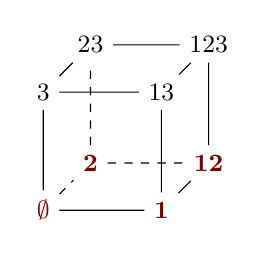
\begin{tikzpicture}[scale=1.5]
    \node [mred] (0) at (0, 0) {\small$\mathbf{\emptyset}$};
    \node [mred] (1) at (1, 0) {\small$\mathbf{1}$};
    \node (3) at (0, 1) {\small$3$};
    \node [mred] (2) at (0.4, 0.4) {\small$\mathbf{2}$};
    \node [mred] (12) at (1.4, 0.4) {\small$\mathbf{12}$};
    \node (13) at (1, 1) {\small$13$};
    \node (23) at (0.4, 1.4) {\small$23$};
    \node (123) at (1.4, 1.4) {\small$123$};

    \draw (0) -- (1) -- (12) -- (123) -- (23) -- (3) -- (0);
    \draw (3) -- (13) -- (1);
    \draw (13) -- (123);

    \draw [dashed] (0) -- (2) -- (12);
    \draw [dashed] (2) -- (23);
  \end{tikzpicture}
\end{center}

For $n = 4$, we can take $\{\emptyset, 1, 2, 3, 4, 12, 13, 23\}$, which is again compressed by not an initial segment. It is an initial segment only if we replace $23$ with $14$.
\begin{center}
  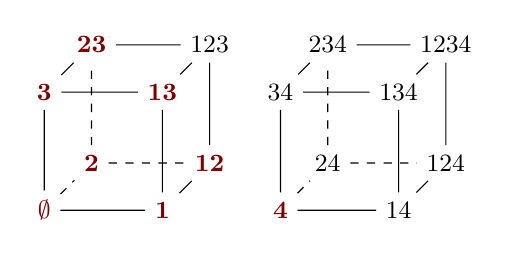
\begin{tikzpicture}[scale=1.5]
    \node [mred] (0) at (0, 0) {\small$\mathbf{\emptyset}$};
    \node [mred] (1) at (1, 0) {\small$\mathbf{1}$};
    \node [mred] (3) at (0, 1) {\small$\mathbf{3}$};
    \node [mred] (2) at (0.4, 0.4) {\small$\mathbf{2}$};
    \node [mred] (12) at (1.4, 0.4) {\small$\mathbf{12}$};
    \node [mred] (13) at (1, 1) {\small$\mathbf{13}$};
    \node [mred] (23) at (0.4, 1.4) {\small$\mathbf{23}$};
    \node (123) at (1.4, 1.4) {\small$123$};

    \draw (0) -- (1) -- (12) -- (123) -- (23) -- (3) -- (0);
    \draw (3) -- (13) -- (1);
    \draw (13) -- (123);
    \draw [dashed] (0) -- (2) -- (12);
    \draw [dashed] (2) -- (23);

    \begin{scope}[shift={(2, 0)}]
    \node [mred] (0) at (0, 0) {\small$\mathbf{4}$};
    \node (1) at (1, 0) {\small$14$};
    \node (3) at (0, 1) {\small$34$};
    \node (2) at (0.4, 0.4) {\small$24$};
    \node (12) at (1.4, 0.4) {\small$124$};
    \node (13) at (1, 1) {\small$134$};
    \node (23) at (0.4, 1.4) {\small$234$};
    \node (123) at (1.4, 1.4) {\small$1234$};

    \draw (0) -- (1) -- (12) -- (123) -- (23) -- (3) -- (0);
    \draw (3) -- (13) -- (1);
    \draw (13) -- (123);
    \draw [dashed] (0) -- (2) -- (12);
    \draw [dashed] (2) -- (23);

    \end{scope}
  \end{tikzpicture}
\end{center}
We notice that these two examples have a common pattern. The ``swap'' we have to perform to get to an initial segment is given by replacing an element with its complement, or equivalently, swapping something the opposite diagonal element. This is indeed general.
\begin{lemma}
  For each $n$, there exists a unique element $z \in Q_n$ such that $z^c$ is the successor of $z$.

  Moreover, if $B \subseteq Q_n$ is compressed but not an initial segment, then $|B| = 2^{n - 1}$ and $B$ is obtained from taking the initial segment of size $2^{n - 1}$ and replacing $x$ with $x^c$.
\end{lemma}

\begin{proof}
  For the first part, simply note that complementation is an order-reversing bijection $Q_n \to Q_n$, and $|Q_n|$ is even. So the $2^{n - 1}$th element is the only such element $z$.

  Now if $B$ is not an initial segment, then we can find some $x < y$ such that $x \not \in B$ and $y \in B$. Since $B$ is compressed, it must be the case that for each $i$, there is exactly one of $x$ and $y$ that contains $i$. Hence $x = y^c$. Note that this is true for all $x < y$ such that $x \not \in B$ and $y \in B$. So if we write out the simplicial order, then $B$ must look like
  \begin{center}
    \begin{tikzpicture}[scale=0.5]
      \foreach \x in {0,...,7} {
        \fill (\x, 0) circle [radius=0.1];
      }
      \draw (8, 0) circle [radius=0.1];
      \fill (9, 0) circle [radius=0.1];
      \foreach \x in {10,...,15} {
        \draw (\x, 0) circle [radius=0.1];
      }
      \node at (16.5, 0) {$\cdots$};
    \end{tikzpicture}
  \end{center}
 since any $x \not \in B$ such that $x < y$ must be given by $x = y^c$, and so there must be a unique such $x$, and similarly the other way round. So it must be the case that $y$ is the successor of $x$, and so $x = z$.
\end{proof}
We observe that these anomalous compressed sets are worse off than the initial segments (exercise!). So we deduce that

%We define these exception sets for $n \geq 3$. For $n = 2k + 1$, we define
%\[
%  B_n^* = \left(X^{(\leq k)} \setminus \{\{(k + 2)(k + 3) \cdots (2k + 1)\} \}\right) \cup \{12\cdots (k + 1)\}.
%\]
%For $n = 2k$, define
%\[
%  B_n^* = \left(X^{(\leq k - 1)} \cup \{(X \setminus \{1\})^{(k - 1)} + 1\} \setminus \{1 (k + 2) \cdots (2k)\}\right) \cup \{23 \cdots (k + 1)\}.
%\]

\begin{thm}[Harper, 1967]
  Let $A \subseteq Q^n$, and let $C$ be the initial segment in the simplicial order with $|C| = |A|$. Then $|N(A)| \geq |N(C)|$. In particular,
  \[
    |A| = \sum_{i = 0}^r \binom{n}{i}\text{ implies } |N(A)| \geq \sum_{i = 0}^{r + 1} \binom{n}{i}.
  \]
\end{thm}

\subsubsection*{The edge isoperimetric inequality in the cube}
Let $A \subseteq V$ be a subset of vertices in a graph $G = (V, E)$. Consider the \term{edge boundary}
\[
  \partial_e A = \{xy \in E: x \in A, y \not \in A\}.
\]
Given a graph $G$, and given the size of $A$, can we give a lower bound for the size of $\partial_e A$?

\begin{eg}
  Take $G = Q_3$. For the vertex isoperimetric inequality, our optimal solution with $|A| = 4$ was given by
  \begin{center}
    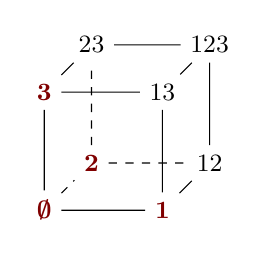
\begin{tikzpicture}[scale=1.5]
      \node [mred] (0) at (0, 0) {\small$\boldsymbol{\emptyset}$};
      \node [mred] (1) at (1, 0) {\small$\mathbf{1}$};
      \node [mred] (3) at (0, 1) {\small$\mathbf{3}$};
      \node [mred] (2) at (0.4, 0.4) {\small$\mathbf{2}$};
      \node (12) at (1.4, 0.4) {\small$12$};
      \node (13) at (1, 1) {\small$13$};
      \node (23) at (0.4, 1.4) {\small$23$};
      \node (123) at (1.4, 1.4) {\small$123$};

      \draw (0) -- (1) -- (12) -- (123) -- (23) -- (3) -- (0);
      \draw (3) -- (13) -- (1);
      \draw (13) -- (123);

      \draw [dashed] (0) -- (2) -- (12);
      \draw [dashed] (2) -- (23);
    \end{tikzpicture}
  \end{center}
  The edge boundary has size $6$. However, if we just pick a slice, then the edge boundary has size $4$ only.
\end{eg}
More generally, consider $Q_n = Q_{2k + 1}$, and take the Hamming ball $B_k = X^{(\leq \ell)}$. Then
\[
  \partial_e B_k = \{AB: A \subseteq B \subseteq X: |A| = k, |B| = k + 1\}.
\]
So we have
\[
  |\partial_e B_k| = \binom{2k + 1}{k + 1} \cdot (k + 1) \sim \frac{2^n \sqrt{n}}{\sqrt{2\pi}}.
\]
However, if we pick the bottom face of $Q_n$. Then $|A| = 2^{n - 1}$ and $|\partial_e A| = 2^{n - 1}$. This is much much better.

More generally, it is not unreasonable to suppose that sub-cubes are always the best. For a $k$-dimensional sub-cube in $Q_n$, we have
\[
  |\partial_k| = 2^k (n - k).
\]
If we want to prove this, and also further solve the problem for $|A|$ not a power of $2$, then as our previous experience would suggest, we should define an order on $\mathcal{P}(X)$.

\begin{defi}[Binary order]\index{binary order}
  The binary order on $Q_n \cong \mathcal{P}(X)$ is given by $x < y$ if $\max x \Delta y \in y$.

  Equivalently, define $\varphi: \mathcal{P}(X) \to \N$ by
  \[
    \varphi(x) = \sum_{i \in x} 2^i.
  \]
  Then $x < y$ if $\varphi(x) < \varphi(y)$.
\end{defi}
The idea is that we avoid large elements. The first few elements in the elements would like like
\[
  \emptyset, 1, 2, 12 3, 13, 23, 123, \ldots.
\]
\begin{thm}
  Let $A \subseteq Q_n$ be a subset, and let $C \subseteq Q_n$ be the initial segment of length $|A|$ in the binary order. Then $|\partial_e C| \leq |\partial_e A|$.
\end{thm}

\begin{proof}
  We induct on $n$ using codimension-$1$ compressions. Recall that we previously defined the sets $A_{\pm}^{(i)}$.

  The $i$-compression of $A$ is the set $B \subseteq Q_n$ such that $|B_{\pm}^{(i)}| = |A_{\pm}^{(i)}|$, and $B_{\pm}^{(i)}$ are initial segments in the binary order. We set $D_i(A) = B$.

  Observe that performing $D_i$ reduces the edge boundary. Indeed, given any $A$, we have
  \[
    |\partial_e A| = |\partial_e A_+^{(i)}| + |\partial_e A_-^{(i)}| + |A_+^{(i)} \Delta A_i^{(i)}|.
  \]
  Applying $D_i$ clearly does not increase any of those factors. So we are happy. Now note that if $A \not= D_i A$, then
  \[
    \sum_{x \in A} \sum_{i \in x} 2^i < \sum_{x \in D_i A} \sum_{i \in x} 2^i.
  \]
  So after applying compressions finitely many times, we are left with a compressed set.

  We now hope that a compressed subset must be an initial segment, but this is not quite true.
  \begin{claim}
    If $A$ is compressed but not an initial, then
    \[
      A = \tilde{B} = \P(X \setminus \{n\}) \setminus \{123\cdots (n-1)\} \cup \{n\}.
    \]
  \end{claim}
  By direct computation, we have
  \[
    |\partial_e \tilde{B}| = 2^{n - 1} - 2(n - 2),
  \]
  and so the initial segment is better. So we are done.

  The proof of the claim is the same as last time. Indeed, by definition, we can find some $x < y$ such that $x \not \in A$ and $y \in A$. As before, for any $i$, it cannot be the case that both $x$ and $y$ contain $i$ or neither contain $i$, since $A$ is compressed. So $x = y^c$, and we are done as before.
\end{proof}

\section{Sum sets}
Let $G$ be an abelian group, and $A, B \subseteq G$. Define
\[
  A + B = \{a + b: a \in A, b \in B\}.
\]
For example, suppose $G = \R$ and $A = \{a_1 < a_2 < \cdots < a_n\}$ and $B = \{b_1 < b_2 < \cdots < b_m\}$. Surely, $A + B \leq nm$, and this bound can be achieved. Can we bound it from below? The elements
\[
  a_1 + b_1, a_1 + b_2, \ldots, a_1 + b_m, a_2 + b_m, \ldots, a_n + b_m
\]
are certainly distinct as well, since they are in strictly increasing order. So
\[
  |A + B| \geq m + n - 1 = |A| + |B| - 1.
\]
What if we are working in a finite group? In general, we don't have an order, so we can't make the same argument. Indeed, the same inequality cannot always be true, since $|G + G| = |G|$. Slightly more generally, if $H$ is a subgroup of $G$, then $|H + H| = |H|$.

So let's look at a group with no subgroups. In other words, pick $G = \Z_p$.

\begin{thm}[Cauchy--Davenport theorem]\index{Cauchy--Davenport theorem}
  Let $A$ and $B$ be non-empty subsets of $\Z_p$ with $p$ a prime, and $|A| + |B| \leq p + 1$. Then
  \[
    |A + B| \geq |A| + |B| - 1.
  \]
\end{thm}

\begin{proof}
  We may assume $1 \leq |A| \leq |B|$. Apply induction on $|A|$. If $|A| = 1$, then there is nothing to do. So assume $A \geq 2$.

  Since everything is invariant under translation, we may assume $0, a \in A$ with $a \not= 0$. Then $\{a, 2a, \ldots, pa\} = \Z_p$. So there exists $k \geq 0$ such that $ka \in B$ and $(k + 1) a \not \in B$.

  By translating $B$, we may assume $0 \in B$ and $a \not \in B$.

  Now $0 \in A \cap B$, while $a \in A \setminus B$. Therefore we have
  \[
    1 \leq |A \cap B| < |A|.
  \]
  Hence
  \[
    |(A \cap B) + (A \cup B)| \geq |A \cap B| + |A \cup B| - 1 = |A| + |B| - 1.
  \]
  Also, clearly
  \[
    (A \cap B) + (A \cup B) \subseteq A + B.
  \]
  So we are done.
\end{proof}

\begin{cor}
  Let $A_1, \ldots, A_k$ be non-empty subsets of $\Z_p$ such that
  \[
    \sum_{i =1 }^d |A_i| \leq p + k - 1.
  \]
  Then
  \[
    |A_1 + \ldots + A_k| \geq \sum_{i = 1}^k |A_i| - k + 1.
  \]
\end{cor}
What if we don't take sets, but sequences? Let $a_1, \ldots, a_m \in \Z_n$. What $m$ do we need to take to guarantee that there are $m$ elements that sums to $0$? By the pigeonhole principle, $m \geq n$ suffices. Indeed, consider the sequence
\[
  a_1, a_1 + a_2, a_1 + a_2 + a_3, \cdots, a_1 + \cdots + a_n.
\]
If they are all distinct, then one of them must be zero, and so we are done. If they are not distinct, then by the pigeonhole principle, there must be $k < k'$ such that
\[
  a_1 + \cdots + a_k = a_1 + \cdots + a_{k'}.
\]
So it follows that
\[
  a_{k + 1} + \cdots + a_{k'}.
\]
So in fact we can even require the elements we sum over to be consecutive. On the other hand, $m \geq n$ is also necessary, since we can take $a_i = 1$ for all $i$.

We can tackle a harder question, where we require that the sum of a fixed number of things vanishes.
\begin{thm}[Erd\"os--Ginzburg--Ziv]
  Let $a_1, \ldots, a_{2n - 1} \in \Z_n$. Then there exists $I \in [2n - 1]^{(n)}$ such that
  \[
    \sum_{i \in I} a_i = 0
  \]
  in $\Z_n$.
\end{thm}

\begin{proof}
  First consider the case $n = p$ is a prime. Write
  \[
    0 \leq a_1 \leq a_2 \leq \cdots \leq a_{2p - 1} < p.
  \]
  If $a_i = a_{i + p - 1}$, then there are $p$ terms that are the same, and so we are done by adding them up. Otherwise, set $A_i = \{a_i, a_{i + p - 1}\}$ for $i = 1, \ldots, p - 1$, and $A_p = \{a_{2p - 1}\}$, then $|A_i| = 2$ for $i = 1, \ldots, p - 1$ and $|A_p| = 1$. Hence we know
  \[
    |A_1 + \cdots + A_p| \geq (2(p - 1) + 1) - p + 1 = p.
  \]
  Thus, every element in $\Z_p$ is a sum of some $p$ of our terms, and in particular $0$ is.

  In general, suppose $n$ is not a prime. Write $n = pm$, where $p$ is a prime and $m > 1$. By induction, for every $2m - 1$ terms, we can find $m$ terms whose sum is a multiple of $m$.

  Select \emph{disjoint} $S_1, S_2, \ldots, S_{2p - 1} \in [2n - 1]^{(m)}$ such that
  \[
    \sum_{j \in S_i} a_j = m b_i.
  \]
  This can be done because after selecting, say, $S_1, \ldots, S_{2p - 2}$, we have
  \[
    (2n - 1) - (2p - 2)m = 2m - 1
  \]
  elements left, and so we can pick the next one.

  We are essentially done, because we can pick $j_1, \ldots, j_p$ such that $\sum_{k = 1}^p b_{i_k}$ is a multiple of $p$. Then
  \[
    \sum_{k = 1}^p \sum_{j \in S_{i_k}} a_j
  \]
  is a sum of $mp = n$ terms whose sum is a multiple of $mp$.
\end{proof}

\section{Projections}
So far, we have been considering discrete objects only. For a change, let's work with something continuous.

Let $K \subseteq \R^n$ be a bounded open set. For $A \subseteq [n]$, we set
\[
  K_A = \{(x_i)_{i \in A} : \exists y \in K, y_i - x_i\text{ for all }i \in A\} \subseteq \R^A.
\]
We write $|K_A|$ for the Lebesgue measure of $K_A$ as a subset of $\R^A$. The question we are interested in is given some of these $|K_A|$, can we bound $|K|$? In some cases, it is completely trivial.
\begin{eg}
  If we have a partition of $A_1 \cup \cdots \cup A_m = [n]$, then we have
  \[
    |K| \leq \prod_{i = 1}^m |K_{A_i}|.
  \]
\end{eg}

But, for example, in $\R^3$, can we bound $|K|$ given $|K_{12}|$, $|K_{13}|$ and $|K_{23}|$?

It is clearly not possible if we only know, say $|K_{12}|$ and $|K_{13}|$. For example, we can consider the boxes
\[
  \left(0, \frac{1}{n}\right) \times (0, n) \times (0, n).
\]
\begin{prop}
  Let $K$ be a body in $\R^3$. Then
  \[
    |K|^2 \leq |K_{12}| |K_{13}| |K_{23}|.
  \]
\end{prop}
This is actually quite hard to prove! However, given what we have done so far, it is natural to try to compress $K$ in some sense. Indeed, we know equality holds for a box, and if we can make $K$ look more like a box, then maybe we can end up with a proof.

For $K \subseteq \R^n$, its \term{$n$-sections} are the sets $K(x) \subseteq \R^{n - 1}$ defined by
\[
  K(x) = \{(x_1, \ldots, x_{n - 1}) \in \R^{n - 1}: (x_1, \ldots, x_{n - 1}, x) \in K\}.
\]
\begin{proof}
  Suppose first that each section of $K$ is a square, i.e.
  \[
    K(x) = (0, f(x)) \times (0, f(x))\;\d x
  \]
  for all $x$ and some $f$. Then
  \[
    |K| = \int f(x)^2\;\d x.
  \]
  Moreover,
  \[
    |K_{12}| = \left(\sup_x f(x)\right)^2 \equiv M^2,\quad |K_{13}| = |K_{23}| = \int f(x)\;\d x.
  \]
  So we have to show that
  \[
    \left(\int f(x)^2\;\d x\right)^2 \leq M^2 \left(\int f(x)\;\d x \right)^2,
  \]
  but this is trivial, because $f(x) \leq M$ for all $x$.

  Let's now consider what happens when we compress $K$. For the general case, define a new body $L \subseteq \R^3$ by setting its sections to be
  \[
    L(x) = (0, \sqrt{|K(x)|}) \times (0, \sqrt{|K(x)|}).
  \]
  Then $|L| = |K|$, and observe that
  \[
    |L_{12}| \leq \sup |K(x)| \leq \left|\bigcup K(x)\right| = |K_{12}|.
  \]
  To understand the other two projections, we introduce
  \[
    g(x) = |K(x)_1|,\quad h(x) = |K(x)_2|.
  \]
  Now observe that
  \[
    |L(x)| = |K(x)| \leq g(x) h(x),
  \]
  Since $L(x)$ is a square, it follows that $L(x)$ has side length $\leq g(x)^{1/2} h(x)^{1/2}$. So
  \[
    |L_{13}| = |L_{23}| \leq \int g(x)^{1/2} h(x)^{1/2}\;\d x.
  \]
  So we want to show that
  \[
    \left(\int g^{1/2}h^{1/2} \;\d x\right)^2 \leq \left(\int g\;\d x\right)\left(\int h\;\d x\right).
  \]
  Observe that this is just the Cauchy--Schwarz inequality applied to $g^{1/2}$ and $h^{1/2}$. So we are done.
\end{proof}

Let's try to generalize this.
\begin{defi}[(Uniform) cover]\index{uniform cover}\index{cover}
  We say a family $A_1, \ldots, A_r \subseteq [n]$ \emph{covers} $[n]$ if
  \[
    \bigcup_{i = 1}^r A_r = [n],
  \]
  and is a \emph{uniform $k$-cover} if each $i \in [n]$ is in exactly $k$ many of the sets.
\end{defi}

\begin{eg}
  With $n = 3$, the singletons $\{1\}, \{2\}, \{3\}$ form a $1$-uniform cover, and so does $\{1\}, \{2, 3\}$. Also, $\{1, 2\}, \{1, 3\}$ and $\{2, 3\}$ form a uniform $2$-cover. However, $\{1, 2\}$ and $\{2, 3\}$ do not form a uniform cover of $[3]$.
\end{eg}
Note that we allow repetitions.
\begin{eg}
  $\{1\}, \{1\}, \{2, 3\}, \{2\}, \{3\}$ is a $2$-uniform cover of $[3]$.
\end{eg}

\begin{thm}[Uniform cover inequality]\index{uniform cover inequality}
  If $A_1, \ldots, A_r$ is a uniform $k$-cover of $[n]$, then
  \[
    |K|^k = \prod_{i = 1}^r |K_A|.
  \]
\end{thm}

\begin{proof}
  Let $\mathcal{A}$ be a $k$-uniform cover of $[k]$. Note that $\mathcal{A}$ is a \emph{multiset}. Write
  \begin{align*}
    \mathcal{A}_- &= \{A \in \mathcal{A}: n \not \in A\}\\
    \mathcal{A}_+ &= \{A \setminus \{n\} \in \mathcal{A}: n \in A\}
  \end{align*}
  We have $|\mathcal{A}_+| = k$, and $\mathcal{A}_+ \cup \mathcal{A}_-$ forms a $k$-uniform cover of $[n - 1]$.

  Now note that if $K = \R^n$ and $n \not \in A$, then
  \[
    |K_A| \geq |K(x)_A|\tag{1}
  \]
  for all $x$. Also, if $n \in A$, then
  \[
    |K_A| = \int |K(x)_{A \setminus \{n\}}|\;\d x.\tag{2}
  \]
  In the previous proof, we used Cauchy--Schwarz. What we need here is H\"older's inequality
  \[
    \int fg\;\d x \leq \left(\int f^p\;\d x\right)^{1/p} \left(\int g^q\;\d x\right)^{1/q},
  \]
  where $\frac{1}{p} + \frac{1}{q} = 1$. Iterating this, we get
  \[
    \int f_1 \cdots f_k\;\d x\leq \prod_{i = 1}^k \left(\int f_i^k\;\d x\right)^{1/k}.
  \]
  Now to perform the proof, we induct on $n$. We are done if $n = 1$. Otherwise, given $K \subseteq \R^n$ and $n \geq 2$, by induction,
  \begin{align*}
    |K| &= \int |K(x)|\;\d x \\
    &\leq \int \prod_{A \in A_-} |K(x)_A|^{1/k} \prod_{A \in \mathcal{A}_+} |K(x)_A|^{1/k}\;\d x\tag{by induction}\\
    &\leq \prod_{A \in \mathcal{A}_-} |K_A|^{1/k} \int \prod_{A \in \mathcal{A}_+}|K(x)_A|^{1/k}\;\d x\tag{by (1)}\\
    &\leq \prod_{A \leq |\mathcal{A}_-} |K_A|^{1/k} \prod_{A \in \mathcal{A}_+} \left(\int |K(x)_A|\right)^{1/k} \tag{by H\"older}\\
    &= \prod_{A \in \mathcal{A}} |K_A|^{1/k} \prod_{A \in \mathcal{A}_+} |K_{A \cup \{n\}}|^{1/k}\tag{by (2)}.%\qedhere
  \end{align*}
\end{proof}
This theorem is great, but we can do better. In fact,

\begin{thm}[Box Theorem (Bollob\'as, Thomason)]\index{box theorem}
  Given a body $K \subseteq \R^n$, i.e.\ a non-empty bounded open set, there exists a box $L$ such that $|L| = |K|$ and $|L_A| \leq |K_A|$ for all $A \subseteq [n]$.
\end{thm}
Of course, this trivially implies the uniform cover theorem. Perhaps more surprisingly, we can deduce this from the uniform cover inequality.

To prove this, we first need a lemma.
\begin{defi}[Irreducible cover]\index{reducible cover}\index{irreducible cover}
  A uniform $k$-cover is \emph{reducible} if it is the disjoint union of two uniform covers. Otherwise, it is \emph{irreducible}.
\end{defi}

\begin{lemma}
  There are only finitely many irreducible covers of $[n]$.
\end{lemma}

\begin{proof}
  Let $\mathcal{A}$ and $\mathcal{B}$ be covers. We say $\mathcal{A} < \mathcal{B}$ if $\mathcal{A}$ is a ``subset'' of $\mathcal{B}$, i.e.\ for each $A \subseteq [n]$, the multiplicity of $A$ in $\mathcal{A}$ is less than the multiplicity in $\mathcal{B}$.

  Then note that the set of irreducible uniform $k$-covers form an anti-chain, and observe that there cannot be an infinite anti-chain.

%  Observe that we can represent families $\mathcal{A}$ by ``indicator functions'' $\psi_\mathcal{A}: \mathcal{P}(n) \to \Z$ by setting $\psi_\mathcal{A}(A)$ to be the multiplicity of $A$ in $\mathcal{A}$. Then we can reformulate the definition of uniform $k$-covers as saying $\psi: \mathcal{P}(n) \to \Z$ satisfies
%  \[
%    \sum_{A : i \in A} \psi(A) = k
%  \]
%  for all $i \in [n]$.
%
%  In this formulation, $\psi$ is reducible if we can write $\psi = \psi_1 + \psi_2$, where $\psi_1$ and $\psi_2$ are both uniform covers.
%
%  Given two covers $\psi_1, \psi_2: \mathcal{P}(n) \to \Z$, we say $\psi_1 < \psi_2$ if $\psi_1(A) < \psi_2(A)$ for all $A$. Then
%
%Fix a finite set $\Omega$, and define an ordering on $\R^\Omega$ by saying $f < g$ if $f(x) < g(x)$ for all $x$.
%
%Can we have an infinite anti-chain $f_1, f_2, \ldots$? One can easily produce such an example! However, we cannot have an infinite anti-chain in $\Z^\Omega$. In fact, we can easily see that there is an increasing subsequence.
%
%Hence, there are only finitely many irreducible uniform $k$ covers of $[n]$. However, we haven't shown any upper bound!
\end{proof}

\begin{proof}[Proof of box theorem]
  For $\mathcal{A}$ an irreducible cover, we have
  \[
    |K|^k \leq \prod_{A \in \mathcal{A}} |K_A|.
  \]
  Also,
  \[
    |K_A| \leq \prod_{i \in A} |K_{\{i\}}|.
  \]
  Let $\{x_A: A \subseteq [n]\}$ be a minimal array with $x_A \leq |K_A|$ such that for each irreducible $k$-cover $\mathcal{A}$, we have
  \[
    |K|^k \leq \prod_{A \in \mathcal{A}} x_A\tag{$1$}
  \]
  and moreover
  \[
    x_A \leq \prod_{i \in A} x_{\{i\}}\tag{$2$}
  \]
  for all $A \subseteq [n]$. We know this exists since there are only finitely many inequalities to be satisfied, and we can just decrease the $x_A$'s one by one. Now again by finiteness, for each $x_A$, there must be at least one inequality involving $x_A$ on the right-hand side that is in fact an equality.

  \begin{claim}
    For each $i \in [n]$, there exists a uniform $k_i$-cover $\mathcal{C}_i$ containing $\{i\}$ with equality
    \[
      |K|^{k_i} = \prod_{A \in \mathcal{C}_i} x_A.
    \]
  \end{claim}

  Indeed if $x_i$ occurs on the right of (1), then we are done. Otherwise, it occurs on the right of (2), and then there is some $A$ such that (2) holds with equality. Now there is some cover $\mathcal{A}$ containing $A$ such that (1) holds with equality. Then replace $A$ in $\mathcal{A}$ with $\{ \{j\}: j \in A\}$, and we are done.

  Now let
  \[
    \mathcal{C} = \bigcup_{i = 1}^n \mathcal{C}_i,\quad
    \mathcal{C}' = \mathcal{C} \setminus \{\{1\}, \{2\}, \ldots, \{n\}\},\quad
    k = \sum_{i = 1}^n k_i.
  \]
  Then
  \[
    |K|^k = \prod_{A \in \mathcal{C}} x_A = \left(\prod_{A \in \mathcal{C}^1} x_A\right)\geq |K|^{k - 1} \prod_{i = 1}^n x_i.
  \]
  So we have
  \[
    |K| \geq \prod_{i = 1}^n x_i.
  \]
  But we of course also have the reverse inequality. So it must be the case that they are equal.

  Finally, for each $A$, consider $\mathcal{A} = \{A\} \cup \{ \{i\} : i \not \in A\}$. Then dividing (1) by $\prod_{i \in A} x_i$ gives us
  \[
    \prod_{i \not \in A} x_i \leq x_A.
  \]
  By (2), we have the inverse equality. So we have
  \[
    x_A = \prod_{i \in A} x_i
  \]
  for all $i$. So we are done by taking $L$ to be the box with side length $x_i$.
\end{proof}

\begin{cor}
  If $K$ is a union of translates of the unit cube, then for any (not necessarily uniform) $k$-cover $\mathcal{A}$, we have
  \[
    |K|^k \leq \prod_{A \in \mathcal{A}} |K_A|.
  \]
\end{cor}
Here a $k$-cover is a cover where every element is covered at least $k$ times.

\begin{proof}
  Observe that if $B \subseteq A$, then $|K_B| \leq |K_A|$. So we can reduce $\mathcal{A}$ to a uniform $k$-cover.
\end{proof}
%
%\begin{cor}
%  Let $S$ be a set of sequences of length $n$ with terms from a finite set $X$. Then every uniform $k$-cover $\mathcal{A}$ of $[n]$ satisfies
%  \[
%    |S|^k \leq \prod_{A \in \mathcal{A}} |S_A|,
%  \]
%  where $S_A$ is the restriction of the sequences in $S$ to $A$ and $|S|$ is the product of elements in $S$.
%\end{cor}

\section{Alon's combinatorial Nullstellensatz}
Alon's combinatorial Nullstellensatz is a seemingly unexciting result that has surprisingly many useful consequences.
\begin{thm}[Alon's combinatorial Nullstellensatz]\index{combinatorial Nullstellensatz}\index{Alon's combinatorial Nullstellensatz}
  Let $\F$ be a field, and let $S_1, \ldots, S_n$ be non-empty finite subsets of $\F$ with $|S_i| = d_i + 1$. Let $f \in \F[X_1, \ldots, X_n]$ have degree $d = \sum_{i = 1}^n d_i$, and let the coefficient of $X_1^{d_1} \cdots X_n^{d_n}$ be non-zero. Then $f$ is not identically zero on $S = S_1 \times \cdots \times S_n$.
\end{thm}

Its proof follows from generalizing facts we know about polynomials in one variable. Here $R$ will always be a ring; $\F$ always a field, and $\F_q$ the unique field of order $q = p^n$. Recall the following result:
\begin{prop}[Division algorithm]\index{division algorithm}
  Let $f, g \in R[X]$ with $g$ monic. Then we can write
  \[
    f = hg + r,
  \]
  where $\deg h \leq \deg f - \deg g$ and $\deg r < \deg g$.
\end{prop}
Our convention is that $\deg 0 = -\infty$.

Let $X = (X_1, \ldots, X_n)$ be a sequence of variables, and write $R[X] = R[X_1, \ldots, X_n]$.

\begin{lemma}
  Let $f \in R[X]$, and for $i = 1, \ldots, n$, let $g_i(X_i) \in R[X_i] \subseteq R[X]$ be monic of degree $\deg g_i = \deg_{X_i} g_i = d_i$. Then there exists polynomials $h_1, \ldots, h_n, r \in R[X]$ such that
  \[
    f = \sum f_i g_i + r,
  \]
  where
  \begin{align*}
    \deg h_i &\leq \deg f - \deg d_i & \deg_{X_i} r &\leq d_i - 1\\
    \deg_{X_i} h_i &\leq \deg_{X_i} f - d_i & \deg_{X_i} r &\leq \deg_{X_i} f\\
    \deg_{X_j} h_i &\leq \deg_{X_j} f & \deg r &\leq \deg f
  \end{align*}
  for all $i, j$.
\end{lemma}

\begin{proof}
  Consider $f$ as a polynomial with coefficients in $R[X_2, \ldots, X_n]$, then divide by $g_1$ using the division algorithm. So we write
  \[
    f = h_1 g_1 + r_1.
  \]
  Then we have
  \begin{align*}
    \deg_{X_1} h_1 &\leq \deg_{X_1} f - d_1 & \deg_{X_1} r_1 &\leq d_1 - 1\\
    \deg h_1 &\leq \deg f & \deg_{X_j} r_1 &\leq \deg_{X_j} f\\
    \deg_{X_j} h_1 &\leq \deg_{X_j}f & \deg r &\leq \deg f.
  \end{align*}
  Then repeat this with $f$ replaced by $r_1$, $g_1$ by $g_2$, and $X_1$ by $X_2$.
\end{proof}

We also know that a polynomial of one variable of degree $n \geq 1$ over a field has at most $n$ zeroes.

\begin{lemma}
  Let $S_1, \ldots, S_n$ be non-empty finite subsets of a field $\F$, and let $h \in \F[X]$ be such that $\deg_{X_i} h < |S_i|$ for $i = 1, \ldots, n$. Suppose $h$ is identically $0$ on $S = S_1 \times \cdots \times S_n \subseteq \F^n$. Then $h$ is the zero polynomial.
\end{lemma}

\begin{proof}
  Let $d_i = |S_i| - 1$. We induct on $n$. If $n = 1$, then we are done. For $n \geq 2$, consider $h$ as a one-variable polynomial in $F[X_1, \ldots, X_{n - 1}]$ in $X_n$. Then we can write
  \[
    h = \sum_{i = 0}^{d_n} g_i(X_1, \ldots, X_{n - 1}) X_m^i.
  \]
  Fix $(x_1, \ldots, x_{n - 1}) \in S_1 \times \cdots S_{n - 1}$, and set $c_i = g_i(x_1, \ldots, x_{n - 1}) \in \F$. Then $\sum_{i = 0}^{d_n} c_i X_n^i$ vanishes on $S_n$. So $c_i = g_i(x_1, \ldots, x_{n - 1}) = 0$ for all $(x_1, \ldots, x_{n - 1}) \in S_1 \times \cdots \times S_{n - 1}$. So by induction, $g_i = 0$. So $h = 0$.
\end{proof}

Another fact we know about polynomials in one variables is that if $f \in \F[X]$ vanishes at $z_1, \ldots, z_n$, then $f$ is a multiple of $\prod_{i = 1}^n (X - z_i)$.
\begin{lemma}
  For $i = 1, \ldots, n$, let $S_i$ be a non-empty finite subset of $\F$, and let
  \[
    g_i(X_i) = \prod_{s \in S_i} (X_i - s) \in \F[X_i] \subseteq F[X].
  \]
  Then if $f \in \F[X]$ is identically zero on $S = S_1 \times \cdots \times S_n$, then there exists $h_i \in \F[X]$, $\deg h_i \leq \deg f - |S_i|$ and
  \[
    f = \sum_{i = 1}^n h_i g_i.
  \]
\end{lemma}

\begin{proof}
  By the division algorithm, we can write
  \[
    f = \sum_{i = 1}^n h_i g_i + r,
  \]
  where $r$ satisfies $\deg_{X_i} r < \deg g_i$. But then $r$ vanishes on $S_1 \times \cdots \times S_n$, as both $f$ and $g_i$ do. So $r = 0$.
\end{proof}

We finally get to Alon's combinatorial Nullstellensatz.
\begin{thm}[Alon's combinatorial Nullstellensatz]\index{combinatorial Nullstellensatz}\index{Alon's combinatorial Nullstellensatz}
  Let $S_1, \ldots, S_n$ be non-empty finite subsets of $\F$ with $|S_i| = d_i + 1$. Let $f \in \F[X]$ have degree $d = \sum_{i = 1}^n d_i$, and let the coefficient of $X_1^{d_1} \cdots X_n^{d_n}$ be non-zero. Then $f$ is not identically zero on $S = S_1 \times \cdots \times S_n$.
\end{thm}

\begin{proof}
  Suppose for contradiction that $f$ is identically zero on $S$. Define $g_i(X_i)$ and $h_i$ as before such that
  \[
    f = \sum h_i g_i.
  \]
  Since the coefficient of $X_1^{d_1} \cdots X_n^{d_n}$ is non-zero in $f$, it is non-zero in some $h_j g_j$. But that's impossible, since
  \[
    \deg h_j \leq \left(\sum_{i = 1}^n d_i \right) - \deg g_j = \sum_{i \not= j} d_i - 1,
  \]
  and so $h_j$ cannot contain a $X_1^{d_1} \cdots \hat{X_j}^{d_j} \cdots X_n^{d_n}$ term.
\end{proof}

Let's look at some applications. Here $p$ is a prime, $q = p^k$, and $\F_q$ is the unique field of order $q$.
\begin{thm}[Chevalley, 1935]
  Let $f_1, \ldots, f_m \in \F_q[X_1, \ldots, X_n]$ be such that
  \[
    \sum_{i = 1}^m \deg f_i < n.
  \]
  Then the $f_i$ cannot have exactly one common zero.
\end{thm}

\begin{proof}
  Suppose not. We may assume that the common zero is $0 = (0, \ldots, 0)$. Define
  \[
    f = \prod_{i = 1}^m (1 - f_i(X)^{q - 1}) - \gamma \prod_{i = 1}^n \prod_{s \in \F_q^\times} (X_i - s),
  \]
  where $\gamma$ is chosen so that $F(0) = 0$, namely the inverse of $\left(\prod_{s \in \F_q^\times} (-s)\right)^m$.

  Now observe that for any non-zero $x$, the value of $f_i(x)^{q - 1} = 1$, so $f(x) = 0$.

  Thus, we can set $S_i = \F_q$, and they satisfy the hypothesis of the theorem. In particular, the coefficient of $X_1^{q - 1} \cdots X_n^{q - 1}$ is $\gamma \not= 0$. However, $f$ vanishes on $\F_q^n$. This is a contradiction.
\end{proof}

It is possible to prove similar results without using the combinatorial Nullstellensatz. These results are often collectively refered to as \term{Chevalley--Warning theorems}.
\begin{thm}[Warning]
  Let $f(X) = f(X_1, \ldots, X_n) \in \F_q[X]$ have degree $< n$. Then $N(f)$, the number of zeroes of $f$ is a multiple of $p$.
\end{thm}

One nice trick in doing these things is that finite fields naturally come with an ``indicator function''. Since the multiplicative group has order $q - 1$, we know that if $x \in \F_q$, then
\[
  x^{q - 1} =
  \begin{cases}
    1 & x \not= 0\\
    0 & x = 0
  \end{cases}.
\]
\begin{proof}
  We have
  \[
    1 - f(x)^{q - 1} =
    \begin{cases}
      1 & f(x) = 0\\
      0 & \text{otherwise}
    \end{cases}.
  \]
  Thus, we know
  \[
    N(f) = \sum_{x \in \F_q^n} (1 - f(x)^{q - 1}) = -\sum_{x \in \F_q^n} f(x)^{q - 1} \in \F_q.
  \]
  Further, we know that if $k \geq 0$, then
  \[
    \sum_{x \in \F_q^n} x^k =
    \begin{cases}
      -1 & k = q - 1\\
      0 & \text{otherwise}
    \end{cases}.
  \]
  So let's write $f(x)^{q - 1}$ as a linear combination of monomials. Each monomial has degree $<n(q - 1)$. So there is at least one $k$ such that the power of $X_k$ in that monomial is $< q - 1$. Then the sum over $X_k$ vanishes for this monomial. So each monomial contributes $0$ to the sum.
\end{proof}

We can use Alon's combinatorial Nullstellensatz to effortlessly prove some of our previous theorems.
\begin{thm}[Cauchy--Davenport theorem]\index{Cauchy--Davenport theorem}
  Let $p$ be a prime and $A, B \subseteq \Z_p$ be non-empty subsets with $|A| + |B| \leq p + 1$. Then $|A + B| \geq |A| + |B| - 1$.
\end{thm}

\begin{proof}
  Suppose for contradiction that $A + B \subseteq C \subseteq \Z_p$, and $|C| = |A| + |B| - 2$. Let's come up with a polynomial that encodes the fact that $C$ contains the sum $A + B$. We let
  \[
    f(X, Y) = \prod_{c \in C} (X + Y - c).
  \]
  Then $f$ vanishes on $A \times B$, and $\deg f = |C|$.

  To apply the theorem, we check that the coefficient of $X^{|A| - 1} Y^{|B| - 1}$ is $\binom{|C|}{|A| - 1}$, which is non-zero in $\Z_p$, since $C < p$. This contradicts Alon's combinatorial Nullstellensatz.
\end{proof}

We can also use this to prove Erd\"os--Ginzburg--Ziv again.
\begin{thm}[Erd\"os--Ginzburg--Ziv]
  Let $p$ be a prime and $a_1, \ldots, a_{2p + 1} \in \Z_p$. Then there exists $I \in [2p - 1]^{(p)}$ such that
  \[
    \sum_{i \in I} a_i = 0\in \Z_p.
  \]
\end{thm}

\begin{proof}
  Define
  \begin{align*}
    f_1(X_1, \ldots, X_{2p - 1}) &= \sum_{i = 1}^{2p - 1} X_i^{p - 1}.\\
    f_2(X_1, \ldots, X_{2p - 1}) &= \sum_{i = 1}^{2p - 1} a_i X_i^{p - 1}.
  \end{align*}
  Then by Chevalley's theorem, we know there cannot be exactly one common zero. But $0$ is one common zero. So there must be another. Take this solution, and let $I = \{i : x_i \not= 0\}$. Then $f_1(X) = 0$ is the same as saying $|I| = p$, and $f_2(X) = 0$ is the same as saying $\sum_{i \in I} a_i = 0$.
\end{proof}

We can also consider restricted sums\index{restricted sum}\index{$\overset{\cdot}{+}$}. We set
\[
  A \overset{\cdot}{+} B = \{a + b: a \in A, b \in B, a \not= b\}.
\]
\begin{eg}
  If $n \not= m$, then
  \begin{align*}
    [n] \overset{\cdot}{+} [m] &= \{3, 4, \ldots, m + n\}\\
    [n] \overset{\cdot}{+} [n] &= \{3, 4, \ldots, 2n - 1\}
  \end{align*}
\end{eg}
From this example, we show that if $|A| \geq 2$, then $|A \overset{\cdot}{+} A|$ can be as small as $2|A| - 3$. In 1964, Erd\"os and Heilbronn
\begin{conjecture}[Erd\"os--Heilbronn, 1964]
  If $2|A|\leq p + 3$, then $|A \overset{\cdot}{+} A| \geq 2|A| - 3$.
\end{conjecture}
This remained open for $30$ years, and was proved by Dias da Silva and Hamidoune. A much much simpler proof was given by Alon, Nathanson and Ruzsa in 1996.
\begin{thm}
  Let $A, B \subseteq \Z_p$ be such that $2 \leq |A| < |B|$ and $|A| + |B| \leq p + 2$. Then $A \overset{\cdot}{+} B \geq |A| + |B| - 2$.
\end{thm}
The above example shows we cannot do better.

\begin{proof}
  Suppose not. Define
  \[
    f(X, Y) = (X - Y) \prod_{c \in C} (X + Y - c),
  \]
  where $A \overset{\cdot}{+} B \subseteq C \subseteq \Z_p$ and $|C| = |A| + |B| - 3$.

  Then $\deg g = |A| + |B| - 2$, and the coefficient of $X^{|A| - 1} Y^{|B| - 1}$ is
  \[
    \binom{|A| + |B| - 3}{|A| - 2} - \binom{|A| + |B| - 3}{|A| - 1} \not= 0.
  \]
  Hence by Alon's combinatorial Nullstellensatz, $f(x, y)$ is not identically zero on $A \times B$. A contradiction.
\end{proof}

\begin{cor}[Erd\"os--Heilbronn conjecture]
  If $A, B \subseteq \Z_p$, non-empty and $|A| + |B| \leq p + 3$, and $p$ is a prime, then $|A \overset{\cdot}{+} B| \geq |A| + |B| - 3$.
\end{cor}

\begin{proof}
  We may assume $2 \leq |A| \leq |B|$. Pick $a \in A$, and set $A' = A \setminus \{a\}$. Then
  \[
    |A \overset{\cdot}{+} B| \geq |A' \overset{\cdot}{+} B| \geq |A'| + |B| - 2 = |A| + |B| - 3.\qedhere
  \]
\end{proof}

Now consider the following problem: suppose we have a circular table $\Z_{2n + 1}$. Suppose the host invites $n$ couples, and the host, being a terrible person, wants the $i$th couple to be a disatnce $d_i$ apart for some $1 \leq d_i \leq n$. Can this be done?

\begin{thm}
  If $2n + 1$ is a prime, then this can be done.
\end{thm}

\begin{proof}
  We may wlog assume the host is at $0$. We want to partition $\Z_p \setminus \{0\} = \Z_p^\times$ into $n$ pairs $\{x_i, x_i + d_i\}$. Consider the polynomial ring $\Z_p[X_1, \ldots, X_n] = \Z_p[X]$. We define
  \[
    f(x) = \prod_i X_i (X_i + d_i) \prod_{i < j} (X_i - X_j)(X_i + d_i - X_j) (X_i - X_j - d_j)(X_i + d_i - X_j - d_j).
  \]
  We want to show this is not identically zero on $\Z_p^n$

  First of all, we have
  \[
    \deg f = 4 \binom{n}{2} + 2n = 2n^2.
  \]
  So we are good. The coefficient of $X_1^{2n} \cdots X_n^{2n}$ is the same as that in
  \[
    \prod X_i^2 \prod_{i < j} (X_i - X_j)^4 = \prod X_i^2 \prod_{i \not= j} (X_i - X_j)^2 = \prod X_i^{2n} \prod_{i \not= j} \left(1 - \frac{X_i}{X_j}\right)^2.
  \]
  This, we are looking for the constant term in
  \[
    \prod_{i \not= j} \left(1 - \frac{X_i}{ X_j}\right)^2.
  \]
  By a question on the example sheet, this is
  \[
    \binom{2n}{2,2,\ldots, 2} \not= 0\text{ in }\Z_p.\qedhere
  \]
\end{proof}

Our final example is as follows: suppose we are in $\Z_p$, and $a_1, \ldots, a_p$ and $c_1, \ldots, c_p$ are enumerations of the elements, and $b_i = c_i - a_i$. Then clearly we have $\sum b_i = 0$. Is the converse true? The answer is yes!
\begin{thm}
  If $b_1, \ldots, b_p \in \Z_p$ are such that $\sum b_i = 0$, then there exists numerations $a_1, \ldots, a_p$ and $b_1, \ldots, b_p$ of the elements of $\Z_p$ such that for each $i$, we have
  \[
    a_i + b_i = c_i.
  \]
\end{thm}

\begin{proof}
  It suffices to show that for all $(b_i)$, there are distinct $a_1, \cdots, a_{p - 1}$ such that $a_i + b_i \not= a_j + b_j$ for all $i \not= j$. Consider the polynomial
  \[
    \prod_{i < j} (X_i - X_j)(X_i + b_i - X_j - b_j).
  \]
  The degree is
  \[
    2 \binom{p - 1}{2} = (p - 1)(p - 2).
  \]
  We then inspect the coefficient of $X_1^{p - 2} \cdots X_{p - 1}^{p - 2}$, and checking that this is non-zero is the same as above.
\end{proof}

\printindex
\end{document}
